% ----------------------------------------------------------
\chapter{Solução do modelo mecânico}
% ----------------------------------------------------------
A solução do modelo mecânico foi feita através do \textit{software} ANSYS, na sua versão 2021R1, e a primeira parte desse capítulo descreve a solução numérica pelo método dos elementos finitos (de forma mais genérica possível) comentando as funcionalidades do ANSYS, quando pertinente. Posteriormente, é dada ênfase na solução numérica do modelo constitutivo do material (que é o foco principal do trabalho) que foi implementado no recurso programável \textit{Usermat}. No final desse capítulo é apresentado o domínio, a discretização da malha e do tempo, as condições de contorno e os parâmetros utilizados nas análises.

\section{Forma fraca das equações de campo}
No contexto da evolução quase estática e da hipótese das pequenas perturbações podem-se escrever as equações de campo na sua forma fraca através do princípio dos trabalhos virtuais. Sendo assim, aplicando um campo de deslocamento virtual $\dul$, cinematicamente admissível, em (\ref{eq:equilibrio_estatico_local}), porém ao longo de todo o volume $\Omega$ tem-se que:
\begin{equation}
	\label{eq:deslocamento_virtual}
	\int_{\Omega} \left(\divl \sigmall + \rho \fl \right)d\Omega \cdot \dul = 0,
\end{equation}
\begin{equation}
	\label{eq:deslocamento_virtual_2}
	\int_{\Omega} \divl \sigmall d\Omega \cdot \dul + \int_{\Omega} \rho \fl d\Omega \cdot \dul = 0.
\end{equation}

Aplicando o Teorema da Divergência no termo mais à esquerda da igualdade (\ref{eq:deslocamento_virtual_2}) obtém-se:
\begin{equation}
	\label{eq:deslocamento_virtual_3}
	\int_{\Omega} \sigmall : \dvarepsilonll d\Omega - \left(\int_{\Omega} \rho \fl \cdot \dul d\Omega + \int_{\partial \Omega} \Tl^d \cdot \dul dS \right) = U_{int} - W_{ext} = 0
\end{equation}

A expressão (\ref{eq:deslocamento_virtual}) é uma equação integral em que, no equilíbrio, o trabalho das forças externas $W_{ext}$ sobre o sistema é totalmente convertido em energia potencial interna $U_{int}$  de deformação.

\section{Notação de Voigt}
Os tensores simétricos de segunda e quarta ordem são comumente representados, respectivamente, por arranjos (\textit{arrays}) vetoriais e matriciais convenientes à álgebra computacional. Dessa forma é utilizada a seguinte notação \cite[p. 682]{Zienkiewicz2005}:
\begin{equation}
	\label{eq:sigmal}
	\sigmall \rightarrow \sigmal = \left\{\sigma_{11}~~~\sigma_{22}~~~\sigma_{33}~~~\sigma_{12}~~~\sigma_{23}~~~\sigma_{13} \right\}^T
\end{equation}
\begin{equation}
	\label{eq:varepsilonl}
	\varepsilonll \rightarrow \varepsilonl = \left\{\varepsilon_{11}~~~\varepsilon_{22}~~~\varepsilon_{33}~~~2\varepsilon_{12}~~~2\varepsilon_{23}~~~2\varepsilon_{13} \right\}^T
\end{equation}
\begin{equation}
	\label{eq:Dl}
	\Dllll \rightarrow \Dll = 
	\begin{bmatrix}
		D_{1111} & D_{1122} & D_{1133}  & D_{1112} & D_{1123} & D_{1113} \\
		D_{2211} & D_{2222}  & D_{2233}  & D_{2212} & D_{2223} & D_{2213}  \\
		D_{3311} & D_{3322} & D_{3333}  & D_{3312} & D_{3323} & D_{3313}  \\
		D_{1211} & D_{1222}	& D_{1233}  & D_{1212} & D_{1223} & D_{1213}  \\
		D_{2311} & D_{2322} & D_{2333} & D_{2312} & D_{2323} & D_{2313}  \\
		D_{1311} & D_{1322}	& D_{1333} & D_{1312} & D_{1323} & D_{1313} 
	\end{bmatrix}
\end{equation}
\begin{equation}
	\label{eq:dgdsl}
	\dgdsll \rightarrow \dgdsl = \left\{\dfrac{\partial g}{\partial \sigma_{11}}~~~\dfrac{\partial g}{\partial \sigma_{22}}~~~\dfrac{\partial g}{\partial \sigma_{33}}~~~\dfrac{\partial g}{\partial \sigma_{12}}~~~\dfrac{\partial g}{\partial \sigma_{23}}~~~\dfrac{\partial g}{\partial \sigma_{13}} \right\}^T
\end{equation}
\begin{equation}
	\label{eq:Uml}
	\Umll \rightarrow \Uml = \left\{1~~~1~~~1~~~0~~~0~~~0 \right\}^T
\end{equation}
\begin{equation}
	\label{eq:UmllotimesUll}
	\Umllll \rightarrow \Umll = 
	\begin{bmatrix}
		1 & 0 & 0 & 0 & 0 & 0 \\
		0 & 1 & 0 & 0 & 0 & 0  \\
		0 & 0 & 1 & 0 & 0 & 0  \\
		0 & 0 & 0 & 1/2 & 0 & 0  \\
		0 & 0 & 0 & 0 & 1/2 & 0  \\
		0 & 0 & 0 & 0 & 0 & 1/2 
	\end{bmatrix}
\end{equation}
\begin{equation}
	\label{eq:UmllotimesUll}
	\Umll \otimes \Umll \rightarrow  
	\begin{bmatrix}
		1 & 1 & 1 & 0 & 0 & 0 \\
		1 & 1 & 1 & 0 & 0 & 0  \\
		1 & 1 & 1 & 0 & 0 & 0  \\
		0 & 0 & 0 & 0 & 0 & 0  \\
		0 & 0 & 0 & 0 & 0 & 0  \\
		0 & 0 & 0 & 0 & 0 & 0 
	\end{bmatrix}
\end{equation}
sendo o subscrito $T$ a operação de transposição. Como se pode ver é utilizada a mesma simbologia de tensores de primeira ordem e de segunda ordem representando vetores (arranjos unidimensionais) e matrizes (arranjos bidimensionais), respectivamente. Nessa notação, as operações também são transformadas, de tal forma que:
\begin{equation}
	\label{eq:operacoes_voigt}
	\begin{array}{lcl}
		\underline{a} \cdot \underline{b} \rightarrow \underline{b}^T \underline{a}, \\ 
		\underline{\underline{a}} : \underline{\underline{b}} \rightarrow \underline{a}^T \underline{b}, \\ 
		\underline{\underline a} \otimes \underline{\underline b} \rightarrow \underline a ~ \underline b ^T, \\ 
		\underline{\underline{\underline{\underline{C}}}} : \underline{\underline{b}} \rightarrow \underline{\underline C} ~ \underline b, \\ 
		\underline{\underline{b}}:\underline{\underline{\underline{\underline{C}}}} : \underline{\underline{b}} \rightarrow \underline {b}^T \underline{\underline{C}} ~ \underline{b}, \\ 
		\left( 	\underline{\underline{\underline{\underline{C}}}}:\underline{\underline{a}} \right) \otimes \left( \underline{\underline{b}} :	\underline{\underline{\underline{\underline{C}}}} \right) \rightarrow \underline{\underline{C}}~ \underline{a}~\underline{b}^T \underline{\underline{C}}.
	\end{array}
\end{equation}

Essa é a notação adotada para o restante do trabalho. Logo, o teorema dos trabalhos virtuais (\ref{eq:deslocamento_virtual_3}) pode ser reescrito da seguinte forma:
\begin{equation}
	\label{eq:deslocamento_virtual_3}
	\int_{\Omega} \dvarepsilonl^T \sigmal d\Omega - \left(\int_{\Omega} \rho \dul^T \fl d\Omega + \int_{\partial \Omega} \dul^T \Tl^d dS \right) = U_{int} - W_{ext} = 0
\end{equation}
\section{Discretização espacial em elementos finitos}
\label{cap:Discretização espacial em elementos finitos}
A solução por elementos finitos consiste em discretizar o domínio $\Omega$ em um conjunto de elementos contíguos $\Omega_e$, estabelecendo o que se chama de malha de elementos finitos (\autoref{discretizacao_MEF}). Cada elemento da malha tem um formato simples: de linha, de triângulo ou quadrilátero, de tetraedro ou hexaedro, dependendo da dimensão (1D, 2D ou 3D) do domínio a ser discretizado. Cada elemento está conectado a outros elementos compartilhando "nós" sendo que a principal incógnita do problema são os deslocamentos nodais.
\begin{figure}[H]
	\begin{center}
		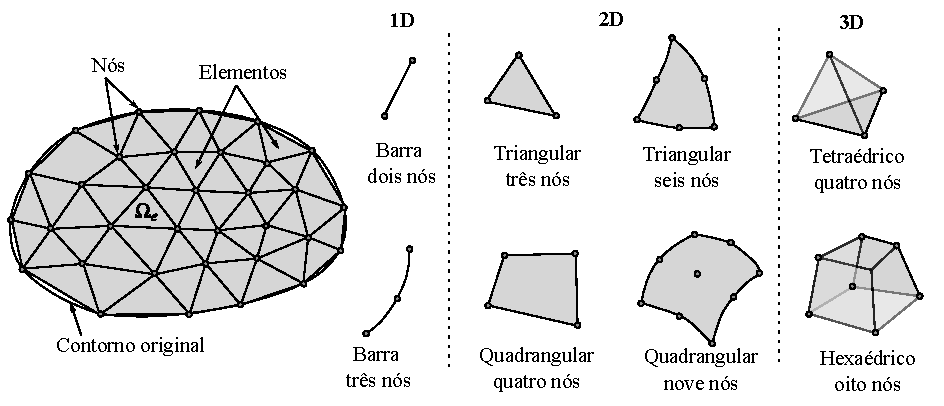
\includegraphics[scale = 1.0]{0601-discretizacao_dominio.pdf}
	\end{center}
	\caption{\label{discretizacao_MEF}Discretização de um domínio genérico em elementos finitos (adaptado de: \citeonline[p. 1-2]{DeSouza2003})}
\end{figure}

Nesse método, o campo de deslocamentos no interior dos elementos é relacionado com os deslocamentos nodais através de funções de interpolação, por exemplo, lineares ou quadráticas, cujos coeficientes são postos em função dos deslocamentos nodais. Dessa forma, o campo de deslocamentos no interior do elemento pode ser descrito como:
\begin{equation}
	\label{eq:campo_deslocamentos}
	\ul(\xl) = \ul(x_1,x_2,x_3) = \Nll(\xl)\ul_e.
\end{equation}
sendo $\ul(\xl)$ o campo de deslocamentos no interior do elemento, $\ul_e$ os deslocamentos nodais e $\Nll$ a matriz contendo as funções de interpolação (também conhecidas como funções de forma). A matriz $\Nll$  tem a seguinte estrutura:
\begin{equation}
	\label{eq:matriz_N}
	\Nll = 	\begin{bmatrix}
		N_1 & 0 & 0 & N_2 & 0 & 0 &  	& N_{n_e} & 0 & 0 \\
		0 & N_1 & 0 & 0 & N_2 & 0 & ... & 0 & N_{n_e} & 0  \\
		0 & 0 & N_1 & 0 & 0 & N_2 &  	& 0 & 0 & N_{n_e} 
	\end{bmatrix}_{n_d \times (n_e \cdot n_d)}
\end{equation}
em que $N_i$ são as funções de interpolação de cada nó $i$, $n_e$ número de nós do elemento e $n_d$ o número de dimensões. Introduzindo (\ref{eq:campo_deslocamentos}) nas equações de compatibilidade (\ref{eq:green_lagrange_linearizado}) tem-se:
\begin{equation}
	\label{eq:deformacoes}
	\varepsilonl(\xl) = \varepsilonl(x_1,x_2,x_3) = \nabla^s\ul(\xl) = \nabla^s \Nll~\ul_e = \Bll~\ul_e
\end{equation}
sendo $\varepsilonl$ o campo de deformações e $\Bll = \nabla^s \Nll$ a matriz que relaciona os deslocamentos nodais com as deformações no interior do elemento. Para problemas tridimensionais, o operador gradiente simétrico $\nabla^s$, na notação de Voigt, é dado por:
\begin{equation}
	\label{eq:gradiente_simetrico}
	\nabla^s = 	\begin{bmatrix}
		\dfrac{\partial}{\partial x_1} & 0 & 0  \\
		0 & \dfrac{\partial}{\partial x_2} & 0  \\
		0 & 0 & \dfrac{\partial}{\partial x_3} \\
		\dfrac{\partial}{\partial x_2} & \dfrac{\partial}{\partial x_1} & 0 \\
		0 & \dfrac{\partial}{\partial x_3} & \dfrac{\partial}{\partial x_2} \\
		\dfrac{\partial}{\partial x_3} & 0 & \dfrac{\partial}{\partial x_1}		
	\end{bmatrix}_{n_c \times n_d}
\end{equation}
em que $n_c$  é o número de componentes de deformações. Introduzindo (\ref{eq:deformacoes}) na lei de comportamento do material, é possível determinar as tensões no interior do elemento também em função dos deslocamentos nodais:
\begin{equation}
	\label{eq:tensoes}
	\sigmal(\xl) = \sigmal(x_1,x_2,x_3) = \Dll ~ \Bll ~\ul_e + \Dll ~\varepsilonl_0 + \sigmal_0
\end{equation}
na qual $\varepsilonl_0$ e $\sigmal_0$ são deformações e tensões iniciais no interior do elemento, respectivamente. Nos problemas de túneis, é através de $\sigmal_0$ que é introduzido as tensões \textit{in situ}. Para o caso de tensão geostática hidrostática, em um túnel de profundidade $H$ em um maciço com peso específico $\gamma_m$ a seguinte expressão é utilizada:
\begin{equation}
	\label{eq:tensoes_iniciais}
	\sigmal_0 = \gamma_m H \Uml
\end{equation}

Introduzindo as expressões (\ref{eq:campo_deslocamentos}), (\ref{eq:deformacoes}) e (\ref{eq:tensoes}) no princípio dos trabalhos virtuais (\ref{eq:deslocamento_virtual_3}), considerando o domínio de um elemento $\Omega_e$, obtém-se a seguinte equação de equilíbrio em forças:
\begin{equation}
	\label{eq:forcas_interna_externa}
	\Fl_{int_e} - \Fl_{ext_e} = \underline 0
\end{equation}
em que:
\begin{equation}
	\label{eq:forca_interna}
	\Fl_{int_e} = \int_{\Omega_e} \Bll^T \sigmal d\Omega_e = \Kll_e \ul_e + \Fl_{\varepsilon_{0_e}} + \Fl_{\sigma_{0_e}}
\end{equation}
\begin{equation}
	\label{eq:forca_externa}
	\Fl_{ext_e} = \Fl_{V_e} + \Fl_{S_e} + \Fl_{C_e} + \Fl_{N_e}
\end{equation}
nos quais:
\begin{equation}
	\label{eq:elementos_forca_interna}
	\Kll_e = \int_{\Omega_e} \Bll^T \sigmal d\Omega_e,~~~ \Fl_{\varepsilon_{0_e}} = \int_{\Omega_e} \Bll^T \Dll~ \varepsilonl_0 d\Omega_e,~~~ \Fl_{\sigma_{0_e}} = \int_{\Omega_e} \Bll^T \sigma_0 d\Omega_e,
\end{equation}
\begin{equation}
	\label{eq:elementos_forca_externa}
	\Fl_{V_e} = \int_{\Omega_e} \rho \Nll^T \fl d\Omega_e,~~~ \Fl_{S_e} = \int_{\partial \Omega_e} \Nll^T \Tl^d dS_e,~~~
	\Fl_{C_e} = \int_{\partial \Omega_{e}} \Nll^T \Tl^c dS_c,
\end{equation}
sendo que $\Fl_{int_e}$ e $\Fl_{ext_e}$ são as forças internas e externas no elemento, respectivamente, $\Kll_e$ a matriz de rigidez do elemento, $\Fl_{\varepsilon_{0_e}}$ e $\Fl_{\sigma_{0_e}}$  forças internas no elemento devido às deformações inciais e tensões iniciais, respectivamente, $\Fl_{V_e}$ forças de volume do elemento, $\Fl_{S_e}$ forças de superfície no contorno livre do elemento, $\Fl_{C_e}$ forças de contato entre elementos vizinhos e $\Fl_{N_e}$  forças nodais. A Figura 6.2 ilustra as forças externas de um elemento genérico.
\begin{figure}[H]
	\begin{center}
		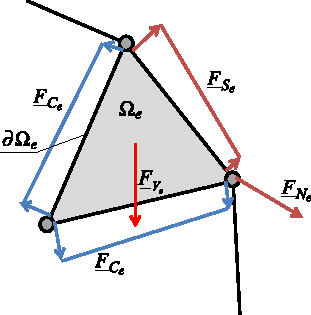
\includegraphics[scale = 1.0]{0602-diagrama de corpo livro de um elemento finito.pdf}
	\end{center}
	\caption{\label{discretizacao_MEF}Diagrama de corpo livre de um elemento finito (adaptado de: \citeonline[p. 19]{Lizarza2011})}
\end{figure}
No método dos elementos finitos, as integrais de volume no domínio  $\Omega_e$, por eficiência, são geralmente resolvidas em um domínio de referência $\Omega_\xi$ com geometria normalizada $-1 \le \xi_i \le 1$. As coordenadas $\underline \xi$ também são conhecidas como coordenadas naturais do elemento. Portanto, é feita a seguinte troca de variáveis nas integrais de volume \cite[p. 147]{Zienkiewicz2005}:
\begin{equation}
	\label{eq:troca_variavel_integral_volume}
	\int_{\Omega_e}d\Omega_e = \iiint dx_1 dx_2 dx_3 = \int_{\Omega_\xi}det(\Jll)d\Omega_\xi = \int_{-1}^{1}\int_{-1}^{1}\int_{-1}^{1}\text{det}(\Jll)d\xi_1d\xi_2d\xi_3
\end{equation}
em que $\Jll = \dfrac{\partial \xl}{\partial \xil}$  é o Jacobiano da transformação entre as coordenada $\xl$ e $\xil$, sendo calculado com as mesmas funções de interpolação usadas para os deslocamentos no interior do elemento, se tratando, portanto, de um \textbf{elemento isoparamétrico}. A integral assim representada é então resolvida pelo método da Quadratura de Gauss-Legendre. Portanto, para uma função $f(\xl)$ qualquer, no domínio $\Omega_e$, tem-se:
\begin{equation}
	\label{eq:troca_variavel_integral_volume}
	\int_{\Omega_e}f(\xl)d\Omega_e = \int_{-1}^{1}\int_{-1}^{1}\int_{-1}^{1}f(\xil)\text{det}(\Jll)d\xi_1d\xi_2d\xi_3 = \sum_{i_p=1}^{n_p}W_{i_p}J_{i_p}f(\xil_{i_p})
\end{equation}
em que $n_p$ é o número de pontos de integração (ou pontos de Gauss), $W_{i_p}$ é o peso referente ao ponto de integração, $f(\xil_{i_p})$ é o valor da função nas coordenadas naturais do ponto de integração e $J_{i_p}$ é o determinante do Jacobiano da transformação (nas coordenadas do ponto de integração) dado por \cite[p. 206-207]{Zienkiewicz2005}:
\begin{equation}
	\label{eq:jacobiano_transformacao}
	J_{i_p} = \left\{
	\begin{array}{lcl}
		 \text{det}(\Jll)_{i_p}~~~\text{em 3D e estado plano de deformações} \\
		2\pi\xi_{r_{i_p}}\text{det}(\Jll)_{i_p} ~~~\text{em axissimetria}
	\end{array}
\right..
\end{equation}
sendo $\xi_{r_{i_p}}$ a coordenada radial natural do ponto de Gauss. A equação (\ref{eq:troca_variavel_integral_volume}) possuí a integração exata se a função for um polinômio de ordem menor ou igual a $2n_p-1$.

Os elementos finitos que são utilizados nesse trabalho com suas funções de interpolação, pesos e coordenadas dos pontos de integração podem ser vistos na \autoref{PLANE183}, para análises em estado plano de deformações e axissimetria e, para análises tridimensionais, que consomem maior tempo de processamento, é utilizado o elemento da \autoref{SOLID185}.
\begin{figure}[H]
	\begin{center}
		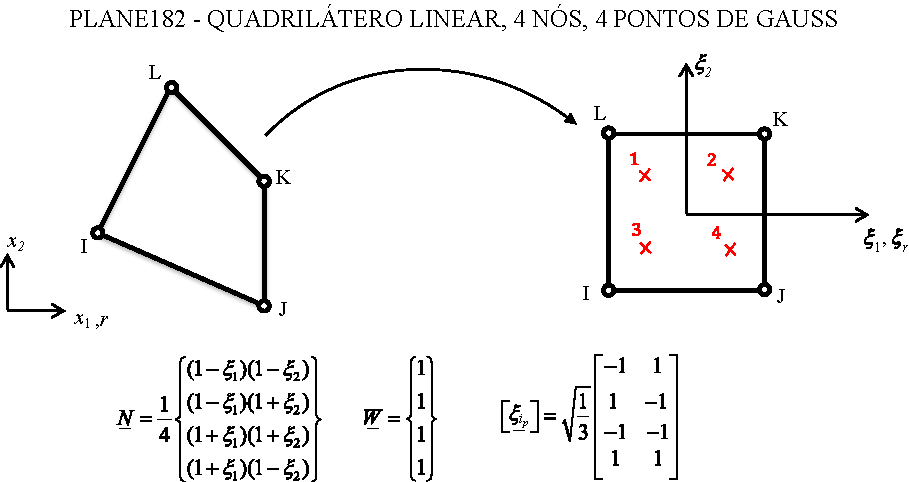
\includegraphics[scale = 1.0]{0603b-quadrilatero linear.pdf}
	\end{center}
	\caption{\label{PLANE183}Funções de interpolação, pesos e coordenadas dos pontos de Gauss para o elemento quadrilátero linear isoparamétrico PLANE182 (adaptado de: \citeonline[p. 334, 369-370]{ANSYS2018})}
\end{figure}
\begin{figure}[H]
	\begin{center}
		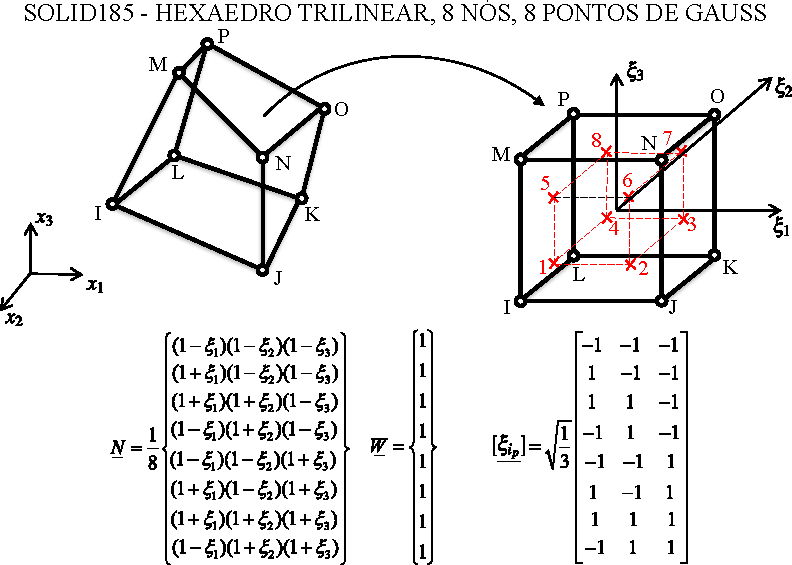
\includegraphics[scale = 1.0]{0604-hexaedro linear.pdf}
	\end{center}
	\caption{\label{SOLID185}Funções de interpolação, pesos e coordenadas dos pontos de Gauss para o elemento hexaedro trilinear isoparamétrico SOLID185 (adaptado de: \citeonline[p. 345, 369-370]{ANSYS2018})}
\end{figure}

No \textit{software} ANSYS, ambos elementos possuem a opção degenerada em que é possível trabalhar de forma colapsada, triangular, por exemplo no caso do elemento PLANE182, e prisma, tetraédrica ou piramidal, no caso do elemento SOLID185. Nas análises apresentadas ao final dessa tese, não foram utilizadas essas formas. Além disso, apesar do \textit{script} APDL ter sido construído com a opção de se trabalhar com os elementos quadráticos (PLANE183 e SOLID186), visando uma melhor eficiência computacional, principalmente para os domínios tridimensionais, optou-se por fazer o estudo de convergência da malha com elementos lineares.

Os elementos PLANE182 e SOLID185 possuem também opções que lidam com problemas de travamento (\textit{Locking}) e modos espúrios (\textit{Hourglass}). O travamento é caracterizado por uma rigidez excessiva do elemento, e ocorre principalmente em elementos de primeira ordem com integração completa que estão sujeitos a flexão. Ou ainda, quando o material é quase incompressível. Também podem ocorrer em elementos de segunda ordem, quando as deformações plásticas são da ordem das deformações elásticas. Esse problema evita-se com refinamento da malha, técnicas de subintegração e funções de formas extras. O ANSYS possuí as duas últimas técnicas para o PLANE182 e SOLID185 (\textit{Uniform Reduced Integration with Hourglass Control} e \textit{Enhanced Strain Formulation}). Já os modos espúrios ocorrem quando se utiliza as técnicas de subintegração e é caracterizado por uma distorção no elemento porém com zero deformação. Esse problema é evitado utilizando integração completa ou refinamento da malha. No presente trabalho utilizou-se a \textbf{integração completa} (\textit{Full integration}) e esses problemas foram evitados com o \textbf{refinamento da malha}. 

\section{Solução do sistema não linear}
\label{cap: solução do sistema}

Após o processo de discretização do domínio $\Omega$ é necessário fazer a montagem e a solução do seguinte sistema global de equações:
\begin{equation}
	\label{eq:sistema_global}
	\left(\Kll~\ul + \Fl_{\varepsilon_{0}} + \Fl_{\sigma_{0}}\right) - \left(\Fl_V+\Fl_S+\Fl_N \right) = \Fl_{int} - \Fl_{ext} = f(\ul) = \underline{0}  
\end{equation}
em que $\Kll$ é a matriz de rigidez global resultante da montagem das matrizes de rigidezes $\Kll_e$ de cada elemento, $\ul$ é o vetor incógnito de deslocamentos nodais global proveniente da montagem dos deslocamentos nodais $\ul_e$ de cada elemento, $\left\{\Fl_V,\Fl_S,\Fl_N,\Fl_{\varepsilon_0},\Fl_{\sigma_0} \right\}$ são as forças globais resultantes da montagem das forças em cada elemento, conforme (\ref{eq:elementos_forca_interna}) e (\ref{eq:elementos_forca_externa}). Evidentemente não há um vetor de forças de contato global $\Fl_C$, uma vez que as forças de contato entre elementos vizinhos possuem a mesma magnitude e sentidos contrários e, portanto, se anulam no somatório global.

Quando há uma não linearidade envolvendo as leis constitutivas do material (tal como na plasticidade ou viscoplasticidade, em que o problema é dependente da trajetória das tensões), a matriz de coeficientes $\Kll$ passa a depender dos deslocamentos nodais incógnitos  $\ul$, tornando o sistema (\ref{eq:sistema_global}) não linear. O \textbf{método de Newton-Raphson} (NR) é o processo iterativo comumente utilizado para resolver esse sistema e é utilizado pelo \textit{software} ANSYS. Dessa forma, aproximando (\ref{eq:sistema_global}) por uma série de Taylor truncada na primeira ordem (linearização) tem-se:
\begin{equation}
	\label{eq:taylor}
	\fl(\ul) \approx \fl(\ul_i) + \fl'(\ul_i)(\ul_{i+1}-\ul_i).
\end{equation}

Fazendo $\fl(\ul) = \underline{0}$, isolando $\ul_{i+1}$ e substituindo (\ref{eq:sistema_global}) em (\ref{eq:taylor}), considerando que $\Fl_{ext}$ não depende dos deslocamentos (devido à hipótese das pequenas perturbações), tem-se a seguinte expressão iterativa para aproximar $\ul$:
\begin{equation}
	\label{eq:NR}
	\ul_{i+1} = \ul_i - \Kll(\ul_i)^{-1}\left(\Fl_{int}(\ul_i)-\Fl_{ext} \right) = \ul_i - \Kll_i^{-1} \left(\Fl_{int_i} - \Fl_{ext} \right) = \ul_i + \Kll_i^{-1}\Rl_i = \ul_i + \Delta \ul_i
\end{equation}
em que $\Delta \ul_i$ é o incremento de deslocamentos nodais da iteração atual $i$, $\Fl_{int_i}$ são as forças internas (ou forças restauradoras) da iteração atual (calculadas com $\ul_i$), $\Rl_i$ é o vetor de carga desbalanceado (também chamado de resíduo) para a iteração atual, $\Kll_i$ a matriz de rigidez global tangente na iteração atual, $\ul_i$ os deslocamentos nodais na iteração atual e $\ul_{i+1}$ os deslocamentos nodais atualizados para a próxima iteração.

Como $\Delta \ul_i = \Kll_i^{-1}\Rl_i$ é um sistema de equações esparso (contém muitos elementos nulos) e geralmente simétrico, há diversas técnicas de solução que buscam explorar essas características para obter eficiência computacional. O \textit{software} ANSYS possui uma técnica de \textbf{solução direta}, que busca resolver o sistema através de operações que compreendem a inversão da matriz de rigidez, e três técnicas de \textbf{soluções indiretas}, que se aproximam da solução do sistema de forma interativa com uma dada tolerância.

A solução direta (\textit{SPARSE - Sparse Direct Solver}) consiste em aplicar a fatorização de Cholesky modificada $\Kll = \Lll~\Dll~ \Lll^T$ (em que $\Lll$ é uma matriz triangular inferior e $\Dll$ uma matriz diagonal) e, através de substituições progressivas e retroativas, resolver o sistema. Em geral, para problemas com poucos graus de liberdade, é uma solução bastante eficiente e não possui problemas de instabilidade numérica. Algoritmos de solução direta análogas podem ser encontrados em \citeonline{Felippa1975} e \citeonline{Smith2014}.

As soluções indiretas, implementadas no ANSYS, se baseiam na família de Métodos dos Gradientes Conjugados Pré-Condicionados, que consistem em minimizar o potencial $V(\Delta \ul) = \frac{1}{2}\Delta \ul^T\Kll~\Delta \ul - \Delta \ul^T\Rl$ com aproximações $\Delta \ul^{(j+1)}=\Delta \ul^{j} + a_j \underline{d}^{(j)}~\text{para}~j=0,1,2,..m$, sendo $\underline d^{(j)}$ os gradientes conjugados, ou seja, $\underline {d}^{{(i)}^T} \Kll d^{(j)} = 0,~~ \forall i \neq j$. Quando o sistema é bem condicionado, sua solução converge para $m \leq n_{gdl}$ iterações e o número de operações é proporcional à raiz quadrada do número de condição da matriz $\Kll$, numero este que é a razão entre o maior e menor autovalor da matriz $\Kll$. Em vista disso, há diversas técnicas de transformação do sistema para melhorar o condicionamento dessa matriz através de uma transformação do tipo $\Mll^{-1}\Kll~\ul = \Mll^{-1} \Rl$, em que $\Mll$ é o pré-condicionador. O ANSYS possuí três métodos implementados \cite[p. 647]{ANSYS2018}:

\begin{alineas}
	
	\item JCG (\textit{Jacobi Conjugate Gradiente}): o pré-condicionador é tomado como sendo uma matriz diagonal cujos termos são as diagonais da matriz de rigidez;
	
	\item ICCG (\textit{Incomplete Cholesky Conjugate Gradiente}), o pré-condicionador é tomado através de uma fatorização incompleta de Cholesky. O algoritmo é internamente desenvolvido pela ANSYS e não publicado, e é mais robusto que o primeiro para matrizes mal condicionadas;
	
	\item PCG (\textit{Preconditioned Conjugate Gradiente}) é um solucionador da \textit{Computational Applications and System Integration, Inc} que não consta nos manuais do \textit{software}. Contudo, é dito eficiente e confiável para problemas mal condicionados.
	
\end{alineas}

Maiores explicações dessas soluções indiretas, podem ser encontrados em \citeonline[p. 316]{Mendonca2019}. Cabe salientar que, tanto os métodos diretos quanto indiretos, são implementados buscando a eficiência computacional, evitando-se trabalhar com os elementos nulos, diminuindo o armazenamento e o número de operações. Alguns métodos que compreendem reordenamento e armazenamento eficiente do sistema, utilizados pelo ANSYS, podem ser encontrados em \citeonline{George1981}. Além disso, uma vantagem do ANSYS é a possibilidade de trabalhar com computação de alto desempenho (\textit{High Performance Computing}) com opções de aceleração usando placas de vídeo da Nvidia, memória compartilhada (SMP - \textit{Shared-Memory Parallel}) ou computação distribuída (MPI - \textit{Message Passing Interface}). Para o presente trabalho, foi utilizado a opção de SMP com 12 processadores.

A rigor para um problema não linear a escolha do melhor método de solução vai depender de testagem. Por padrão o ANSYS utiliza o SPARSE. Contudo, o manual do \textit{software} recomenda utilizar o método PCG para estruturas sólidas 3D que possuem mais de 200.000 graus de liberdade. Para problemas mal condicionados, seja pela forma dos elementos, grandes diferenças entre as propriedades dos materiais ou ainda por insuficiente condições de contorno, recomenda-se o SPARSE \cite[p. 242]{ANSYS2018b}. Esse foi o método de solução escolhido para o presente trabalho.

Para incorporar a dependência do histórico de cargas/tempo, para um dado passo de carga/tempo $p$, a expressão (\ref{eq:NR}) é discretizada em $1 \leq n \leq n_s$ subpassos em que a carga externa e o tempo do passo são incrementados linearmente. Dessa forma, itera-se o sistema (\ref{eq:NR}) repetidas vezes para cada subpasso $n$ tendo-se:
\begin{equation}
	\label{eq:NR1}
	\Delta \ul_{n,i} = \Kll_{n,i}^{-1}\left(\Fl_{ext_{n}} - \Fl_{int_{n,i}} \right) = \Kll_{n,i}^{-1}\Rl_{n,i},
\end{equation}
\begin{equation}
	\label{eq:NR2}
	\ul_{n,i+1} = \ul_{n,i}+\Delta\ul_{n,i},
\end{equation}
\begin{equation}
	\label{eq:NR3}
	\Fl_{ext_{n}} = \Fl_{ext_{n-1}} + \Delta \Fl_{p},
\end{equation}
\begin{equation}
	\label{eq:NR4}
	t_{n} = t_{n-1} + \Delta t_p,
\end{equation}
em que
\begin{equation}
	\label{eq:NR5}
	\Fl_{int_{n,i}} = \left( \int_{\Omega} \Bll^T \sigmal d\Omega \right)_{n,i}
\end{equation}
sendo $\ul_{0,0}$, $\Fl_{int_{0,0}}$, $\Fl_{ext_0}$   e $t_0$ nulos. Para os próximos subpassos os valores de $\ul_{n,0}$ e $\Fl_{int_{n,0}}$, correspondem aos valores da solução convergente no subpasso anterior $n-1$. O número de subpassos $n_s$ e o incremento de força externa $\Delta \underline{F}_p$ são dependentes do incremento de tempo utilizado no passo $\Delta t_p$, e são dados por:
\begin{equation}
	\label{eq:NR6}
	n_s = \dfrac{t_p}{\Delta t_p},~~~ \Delta \Fl_{p} = \dfrac{\Fl_{ext_p}}{n_s}
\end{equation}
sendo $t_p$ e $\Fl_{ext_p}$, nessa ordem, o tempo e a força no final do passo. Em busca da convergência e eficiência computacional, o ANSYS tem a opção de variar automaticamente o $\Delta t_p$ dentro de um intervalo $\Delta t_{p_{min}} \leq \Delta t_p \leq \Delta t_{p_{max}}$ fornecido pelo usuário. É possível que o algoritmo não convirja em um dado subpasso durante as iterações e, portanto, é utilizado um limite de $n_{eqit} = 25$ iterações de equilíbrio por subpasso. Quando a solução não converge dentro desse limite, o ANSYS divide pela metade o incremento de tempo, e consequentemente a carga, e reinicia o cálculo do passo. Esse procedimento é chamado de Método da Bisseção e é executado tantas vezes quanto necessárias até atingir a convergência ou $\Delta t_p \leq \Delta t_{p_{min}}$ a partir do qual a solução é dada como não convergente e estabelecido o critério de parada \cite[p. 637]{ANSYS2018}.

A convergência é verificada sobre o vetor resíduo e o incremento de deslocamentos nodais para cada iteração de equilíbrio, através das seguintes expressões (omitindo-se o subíndice $n$) \cite[p. 667]{ANSYS2018}:
\begin{equation}
	\label{eq:convergencia}
	||\Rl_i|| \leq \varepsilon_R R_{ref},~~~ ||\Delta \ul_i || \leq \varepsilon_u u_{ref}
\end{equation}
em que $\varepsilon_R$ e $\varepsilon_u$ são as tolerâncias para o resíduo (de 0,5\%) e deslocamentos (de 5\%), respectivamente. Os valores de referência $R_{ref}$ e $u_{ref}$ são $||\Fl_{ext_p}||$ e $||\ul_{n,i}||$, respectivamente. Ou seja, por padrão o critério para o resíduo é de 0,5\% do valor das forças externas e o incremento de deslocamentos não podem apresentar um valor maior do que 5\% dos deslocamentos do subpasso. No ANSYS, a norma pode ser calculada de três formas: a máxima componente em valor absoluto, a soma absoluta das componentes ou a norma euclidiana das componentes, conforme:
\begin{equation}
	\label{eq:jacobiano_transformacao}
	||\underline *|| = \left\{
	\begin{array}{lcl}
		||\underline *||_\infty = \text{max}(*_j) \\
		||\underline *||_1 = \sum_{j}|*_j| \\
		||\underline *||_2 = (\sum_{j}*_j^2)^{1/2}
	\end{array}
	\right..
\end{equation}
em que $j$ é o índice da componente do vetor $\underline * = \Rl$ ou $\underline * = \Delta \ul$. Para o presente trabalho foi escolhida a norma euclidiana para o resíduo e a norma infinita para o incremento de deslocamento. A \autoref{NR} ilustra o andamento da solução ao longo dos subpassos. Pode-se ver, caso haja a convergência entre os subpassos, que o resíduo e o incremento de deformações vão ficando cada vez menores ao longo das iterações de equilíbrio.
\begin{figure}[H]
	\begin{center}
		\includegraphics[scale = 1.0]{0605_2-ilustracao das iteracoes do método de NR.pdf}
	\end{center}
	\caption{\label{NR}Ilustração das iterações do método de Newton-Raphson (adaptado de: \citeonline[p. 301]{Chen1988})}
\end{figure}

O ANSYS possui ainda quatro variações do método de Newton-Raphson de acordo com a estratégia de atualização da matriz de rigidez $\Kll_{n,i}$ (\citeyear{ANSYS2018}, p. 666): 
\begin{alineas}
	
	\item \textbf{Completo} (\textit{Full}): quando a matriz de rigidez é atualizada a cada iteração $i$, ou seja, $\Kll_{n,i} \leftarrow \Kll_{n,i}$. Essa opção reduz o número de iterações de equilíbrio (convergência quadrática), porém, exige a montagem, fatorização e inversão da matriz a cada iteração;
	
	\item \textbf{Modificado} (\textit{Modified}): quando a matriz de rigidez é atualizada apenas a cada subpasso de carga/tempo $n$, ou seja, $\Kll_{n,i} \leftarrow \Kll_{n,0}$; 
	
	\item \textbf{Inicial} (\textit{Inicial Stiffness}): quando é utilizada a mesma matriz para todos os subpassos e iterações, ou seja, $\Kll_{n,i} \leftarrow \Kll_{0,0}$. 
	
	\item \textbf{Completo Assimétrico} (\textit{Full with unsymmetric matrix}): atualiza a matriz de rigidez a cada iteração, ou seja, $\Kll_{n,i} \leftarrow \Kll_{n,i}$, porém é utilizada a matriz cheia ao invés de explorar a simetria.
	
\end{alineas}

A convergência quadrática da opção de Newton-Raphson Completo só é efetivamente obtida se for utilizado o módulo consistente $\Dll^{alg}$ após o algoritmo de integração das tensões, conforme \citeonline{Simo1985}. A opção de Newton-Raphson Completo Assimétrico é importante para os casos em que se calcula o módulo consistente e se tem plasticidade não associada. A plasticidade não associada pode levar a módulos constitutivos não simétricos e pode não convergir com o Newton-Raphson Completo, pois este monta a matriz de rigidez considerando-a simétrica. Uma forma de contornar esse problema é não utilizar o módulo consistente, porém serão necessárias mais iterações de equilíbrio para a convergência. Nessa tese, como será visto mais adiante, foi programado o módulo constitutivo consistente, mas o autor optou por manter esse recurso opcional para o usuário.

Apesar de não terem sido utilizadas nessa tese, o ANSYS possui ainda quatro técnicas para melhorar a convergência do método de Newton-Raphson em problemas estáticos, que são \cite[p. 668-673]{ANSYS2018}:

\begin{alineas}
	\item \textbf{Preditor} (\textit{Predictor}): extrapola o vetor de deslocamentos iniciais de cada subpasso utilizando os incrementos de deslocamentos acumulados do subpasso anterior multiplicados pela relação entre os incrementos de tempo de ambos subpassos;
	
	\item \textbf{Descida Adaptativa} (\textit{Adaptative Descent}): consiste em alternar entre a matriz de rigidez tangente e secante conforme o andamento do resíduo durante as iterações de equilíbrio. Só é utilizada em conjunto com o método de Newton-Raphson Completo;
	
	\item \textbf{Pesquisa de linha} (\textit{Line Search}): tenta melhorar a solução multiplicando o incremento de deslocamentos por um escalar determinado pela minimização da energia do sistema;
	
	\item \textbf{Método do comprimento de arco} (\textit{Arc-Length Method}): utilizado para solução de equilíbrio estático não-linear de problemas instáveis como flambagem e pós-flambagem.	
\end{alineas}

Na \autoref{NR-fluxograma} tem-se o fluxograma do método de Newton-Raphson, mostrando as três opções de atualização da matriz de rigidez, o método da bisseção e os laços das iterações de equilíbrio e de subpassos.
\begin{figure}[H]
	\begin{center}
		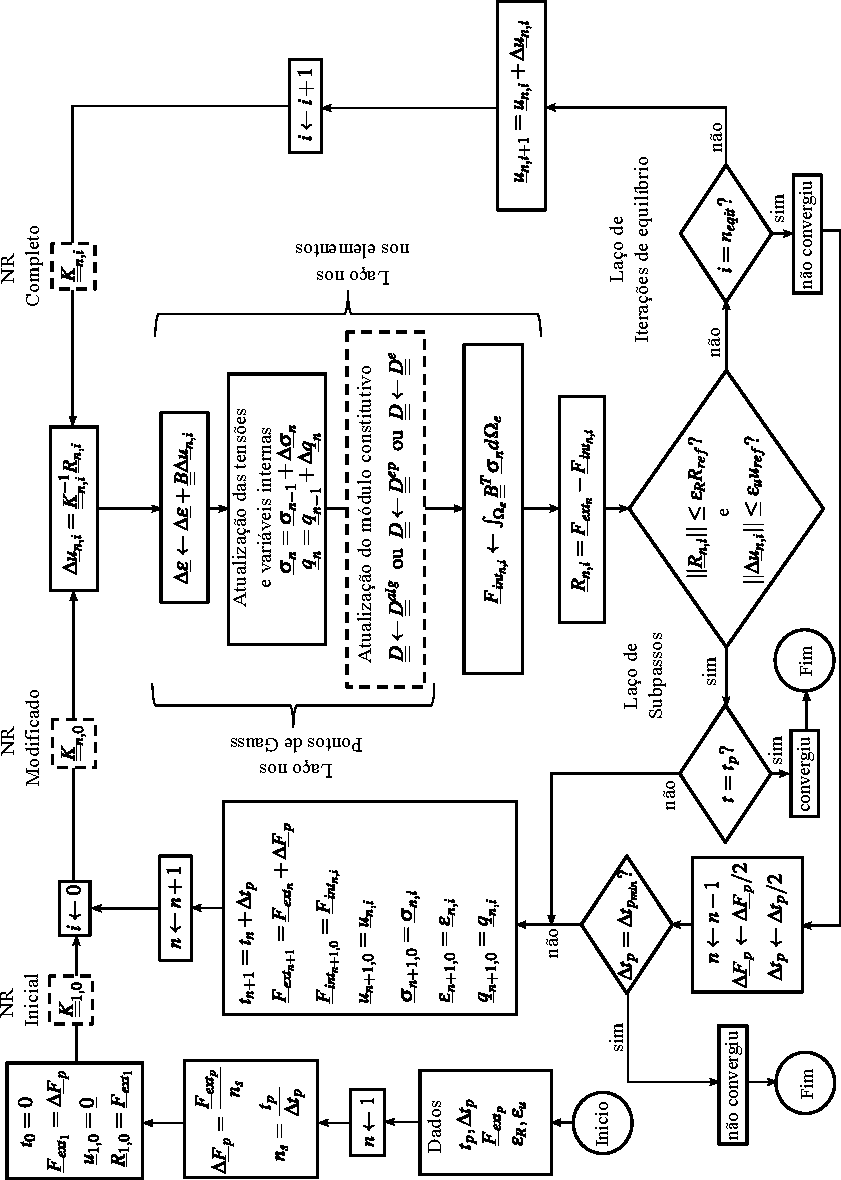
\includegraphics[scale = 1.0]{0606_2-fluxograma do metodo NR.pdf}
	\end{center}
	\caption{\label{NR-fluxograma}Fluxograma do método de Newton-Raphson para solução do sistema de equações globais não lineares}
\end{figure}
Ainda na \autoref{NR-fluxograma} está detalhada a parte de atualização das tensões, variáveis internas e do módulo constitutivo, que serão os temas do próximo capítulo. É importante nesse fluxograma o detalhe dos laços nos elementos e pontos de Gauss, pois a customização do modelo do material, através da subrotina \textit{Usermat}, está justamente aninhada nesse laço mais interno dos pontos de Gauss.

\section{Algoritmo de atualização das tensões e variáveis internas}\label{algoritmo de atualização das tensões e variáveis internas}

Como visto na seção anterior, durante as iterações de equilíbrio é necessário fazer a integração espacial das forças internas no contexto do método dos elementos finitos. Essa integração pode ser escrita da seguinte maneira:
\begin{equation}
	\label{eq:Fint}
	\Fl_{int_{n,i}} = \int_{\Omega}\Bll^T\sigmal_{n}d\Omega = \sum_{i_e=1}^{n_e}\sum_{i_p=1}^{n_p}\left( \Bll^T\sigmal_{n}WJ\right)_{i_p,i_e}
\end{equation}
sendo $\sigmal_{n}$ dado pela relação constitutiva do material. Contudo, as relações constitutivas, por dependerem da trajetória das tensões e/ou do tempo, estão descritas em forma de taxas, conforme visto no \autoref{cap: modelo mecanico}. E, portanto, é necessária a solução desse sistema de equações diferenciais ordinárias por algum método de integração ao longo dos subpassos. Essa etapa de integração, no esquema de elementos finitos, é conhecida como \textbf{algoritmo de atualização das tensões e variáveis internas}. Tal como ilustrado na \autoref{NR-fluxograma}, esse algoritmo ocorre para cada ponto de Gauss de cada elemento e tem por finalidade obter o incremento de tensão $\Delta \sigmal$ e de forças associadas às variáveis internas $\Delta \ql$ através do incremento de deformação total $\Delta \varepsilonl$ do subpasso.

\subsection{Integração das equações constitutivas elastoplásticas}

Como visto no \autoref{cap: modelo mecanico}, considerando a hipótese das pequenas transformações, as equações constitutivas da elastoplasticidade, já na notação de Voigt, podem ser escritas como:
\begin{equation}
	\label{eq:constitutiva_ep}
	\left\{
	\begin{array}{lcl}
		\dot \sigmal = \Dll~\dot \varepsilonl^e = \Dll(\dot \varepsilonl - \dot \varepsilonl^p) \\
		\dot \varepsilonl^p = \dot \lambda \dgdsl \\
		\dot \ql = \dot \lambda \hl \\
		\dot f = \dfdsl^T \dot \sigmal + \dfdql^T \dot \ql = 0 \\
		f \leq 0,~~\dot \lambda \geq 0,~~\dot \lambda f = 0	
	\end{array}
	\right..
\end{equation}

Em geral, a proposta dos algoritmos de integração consiste em integrar as equações constitutivas através de métodos numéricos, como os de Runge-Kutta, com técnicas explícitas, implícitas ou semi-implícitas. E dessa forma, conhecido o conjunto de $\left\{ \varepsilonl_n, \varepsilonl_n^p,\sigmal_n,\ql_n \right\}$ do último subpasso convergido $n$ e o incremento de deformação total acumulado $\Delta \varepsilonl$ obtido pela iteração de Newton-Raphson, busca-se os valores $\left\{ \varepsilonl_{n+1}, \varepsilonl_{n+1}^p,\sigmal_{n+1},\ql_{n+1} \right\}$, plasticamente admissíveis, do subpasso $n+1$. No presente trabalho \textbf{foi implementado um esquema semi-implícito de Euler de dois passos para a relação constitutiva elastoplástica}, inicialmente em elastoplasticidade perfeita, e posteriormente com a lei de endurecimento/amolecimento definida por partes para fins de análise na problemática de túneis.

Em geral, em elastoplasticidade, o método de Runge-Kutta de primeira ordem (também conhecido como o método de Euler) é comumente utilizado para fazer a integração das relações constitutivas (\ref{eq:constitutiva_ep}), tendo-se o seguinte esquema de integração:
\begin{equation}
	\label{eq:esquema_int_constitutiva_ep}
	\left\{
	\begin{array}{lcl}
		\varepsilonl_{n+1} = \varepsilonl_n + \Delta \varepsilonl \\
		\varepsilonl_{n+1}^p = \varepsilonl_n^p + \left[(1-\Theta) \Delta \lambda_n \dgdsl_n + \Theta \Delta \lambda_{n+1} \dgdsl_{n+1}\right] \\
		\ql_{n+1} = \ql_n + \left[(1-\Theta) \Delta \lambda_n \hl_n + \Theta \Delta \lambda_{n+1} \hl_{n+1}\right] \\	
		\sigmal_{n+1} = \Dll~\varepsilonl_{n+1}^e = \Dll( \varepsilonl_{n+1} - \varepsilonl_{n+1}^p) \\
		f_{n+1} = f(\sigmal_{n+1},\ql_{n+1}) = 0		
	\end{array}
	\right.
\end{equation}
em que $\Delta \lambda = \dot\lambda\Delta t$ e $0 \leq \Theta \leq 1$ fornece a regra trapezoidal generalizada para o fluxo plástico e evolução das variáveis internas. Quando $\Theta = 0$ tem-se a forma completamente explicita (\textit{fully explicit forward Euler}) e $\Theta = 1$  completamente implicita (\textit{fully implicit backward Euler}). Os algoritmos semi-implícitos adotam $0 \leq \Theta < 1$  ou ainda uma combinação implícita e explícita de $\Delta \lambda$, $\dgdsl$ e $\hl$.

Os esquemas explícitos, como os de \citeonline{Nayak1972}, \citeonline{Zienkiewicz1969} e \citeonline{Owen1980} foram largamente usados até que \citeonline{Simo1985} propuseram um método implícito de dois passos conhecido como projeção do ponto mais próximo (\textit{Closest Point Projection Method} ou abreviadamente CPPM). Isso pois, os esquemas completamente explícitos não satisfaziam a condição de consistência $f_{n+1} = f(\sigmal_{n+1},\ql_{n+1}) = 0$ no final do subpasso, uma vez que o multiplicador plástico e os vetores de fluxo são calculados com as tensões do subpasso anterior $n$. Segundo \citeonline[p. 278]{Belytschko2000} isso faz com que a solução acumule uma certa imprecisão. Esse fato levou a comunidade a desenvolver e utilizar cada vez mais os algoritmos implícitos e semi-implícitos que buscam satisfazer $f_{n+1} = 0$. E, portanto, é o método adotado nesse trabalho. Alguns dos principais métodos implícitos e semi-implícitos para elastoplasticidade podem ser encontrados em \citeonline{Simo1998}, \citeonline{Belytschko2000}, \citeonline{Neto2008} e \citeonline{Huang2009}.

Atualmente esses métodos empregados nos algoritmos de atualização das tensões consistem em um esquema preditor-corretor de dois passos. Primeiro aplica-se a etapa do preditor elástico e, se necessário, a do corretor plástico. Dessa forma, definindo $\Delta \varepsilonl_{n+1}^p \equiv \varepsilonl_{n+1}^p - \varepsilonl_{n}^p$, o preditor elástico pode ser explicitado de (\ref{eq:esquema_int_constitutiva_ep})$_4$, conforme:
\begin{equation}
	\label{eq:preditor_elastico}
	\sigmal_{n+1} = \Dll(\varepsilonl_{n+1}-\varepsilonl_{n+1}^p) = \Dll(\varepsilonl_n+\Delta \varepsilonl-\varepsilonl_{n}^ p-\Delta \varepsilonl_{n+1}^p) = \sigmal_{n+1}^{trial} + \Delta \sigmal_{n+1}
\end{equation}
em que $\sigmal_{n+1}^{trial} = \Dll(\varepsilonl_n+\Delta \varepsilonl-\varepsilonl_{n}^ p)$ é o \textbf{preditor elástico} (também conhecido como tensão tentativa). Desse modo, no primeiro passo calcula-se a tensão tentativa e testa-se a função de escoamento $f$. Caso $f<0$ o estado de tensões está no domínio elástico e não há necessidade de aplicar o corretor plástico. Contudo, se $f>0$, ou seja, o estado de tensões está fora do domínio plasticamente admissível, é necessário aplicar a etapa do corretor plástico.

O \textbf{corretor plástico}, nada mais é do que o procedimento de solução do sistema (\ref{eq:esquema_int_constitutiva_ep})$_{2,3,5}$ que determinará o valor de $\Delta \sigmal_{n+1}$ e $\Delta \ql_{n+1}$. Quando não é possível obter uma solução analítica para esse sistema, o procedimento de solução comumente utilizado é o de Newton-Raphson que itera $k$ vezes no espaço das tensões e variáveis internas até que o estado de tensões retorne sobre a superfície de escoamento (plasticamente admissível). Por isso esses esquemas também são conhecidos como algoritmos de retorno mapeado (\textit{Return Mapping Algorithm}). A \autoref{algoritmo_retorno} ilustra geometricamente esse procedimento.

\begin{figure}[H]
	\begin{center}
		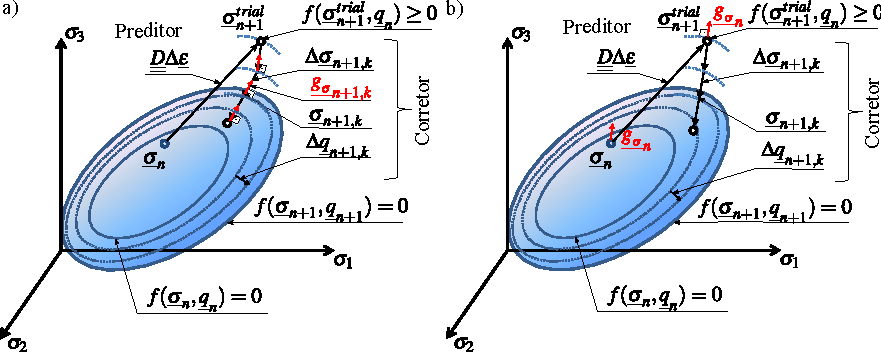
\includegraphics[scale = 1.0]{0607_2-ilustração do algoritmo de retorno.pdf}
	\end{center}
	\caption{\label{algoritmo_retorno}Ilustração do algoritmo de retorno mapeado genérico com $k$ iterações locais de Newton-Raphson: a) totalmente implícito e b) semi-implícito.}
\end{figure}

Uma dificuldade do método totalmente implícito é a necessidade da obtenção de gradientes de segunda ordem das funções potenciais, o que levou ao desenvolvimento e utilização de algoritmos semi-implícitos. No presente trabalho foi implementado o algoritmo de \citeonline{Moran1990} descrito em \citeonline[p. 287]{Belytschko2000} que adotam para o multiplicador plástico um esquema implícito e para o vetor de fluxo e módulo de endurecimento um esquema explícito.

Portanto, para resolver por Newton-Raphson o sistema que dá origem ao corretor plástico, se escrevem as equações (\ref{eq:esquema_int_constitutiva_ep})$_{2,3,5}$ da seguinte forma residual (omitindo-se o índice $n+1$):
\begin{equation}
	\label{eq:algoritmo_ep_1}
	\left\{
	\begin{array}{lcl}
		\al = -\varepsilonl^p + \varepsilonl_n^p + \Delta \lambda \dgdsl_n = \zerol	\\
		\bl = -\ql + \ql_n + \Delta\lambda\hl_n = \zerol \\
		f = f(\sigmal,\ql) = 0
	\end{array}
	\right..
\end{equation}

Linearizando essas equações em relação à $\Delta \lambda$, sendo que $\Delta \varepsilonl^p = - \Dll^{-1}\Delta\sigmal$, tem-se:
\begin{equation}
	\label{eq:algoritmo_ep_2}
	\left\{
	\begin{array}{lcl}
		\al_k + \Dll^{-1}\Delta\sigmal_k + \delta \lambda_k \dgdsl_n = \zerol \\
		\bl_k - \Delta \ql_k + \delta \lambda_k \hl_n = \zerol \\
		f_k + \dfdsl_k^T\Delta\sigmal_k + \dfdql_k^T \Delta \ql_k = 0
	\end{array}
	\right..
\end{equation}

Reorganizando (\ref{eq:algoritmo_ep_2})$_{1,2}$ tem-se o seguinte corretor plástico:
\begin{equation}
	\label{eq:algoritmo_ep_3}
	\left\{
	\begin{array}{lcl}
		\Delta \sigmal_k \\
		\Delta \ql_k
	\end{array}
	\right\} = -\delta\lambda_k \left[ \All \right]
	\left\{	
	\begin{array}{lcl}
		\dgdsl_n \\
		\hl_n
	\end{array}
	\right\}
\end{equation}
em que
\begin{equation}
	\label{eq:Ak}
	\left[ \All \right] =
	\begin{bmatrix}
		\Dll & \zerol \\
		\zerol & -\Uml
	\end{bmatrix}.
\end{equation}

Devido a esse tratamento explícito do vetor de fluxo plástico e do módulo de endurecimento tem-se em (\ref{eq:Ak}) uma expressão fechada para $\left[\All \right]$ envolvendo apenas a matriz constitutiva elástica. Além disso, como o sistema (\ref{eq:algoritmo_ep_2}) é composto de funções lineares em relação à $\Delta \lambda$ os resíduos $\al_k$ e $\bl_k$ serão automaticamente nulos, dispensando sua verificação no critério de convergência. Substituindo (\ref{eq:algoritmo_ep_3}) em (\ref{eq:algoritmo_ep_2})$_3$ tem-se o termo de atualização do multiplicador plástico durante as iterações:
\begin{equation}
	\label{eq:deltalambdak}
	\delta \lambda_k = \dfrac{f_k}{\left[\dfdsl_k^T~~~~\dfdql_k^T\right]\left[\All \right]\left\{ 
	\begin{array}{lcl}
			\dgdsl_n \\ 
			\hl_n
	\end{array}\right\}}
\end{equation}

O fluxograma desse algoritmo pode ser visto na \autoref{algoritmo_EP_semiimplicito}.

\begin{figure}[H]
	\begin{center}
		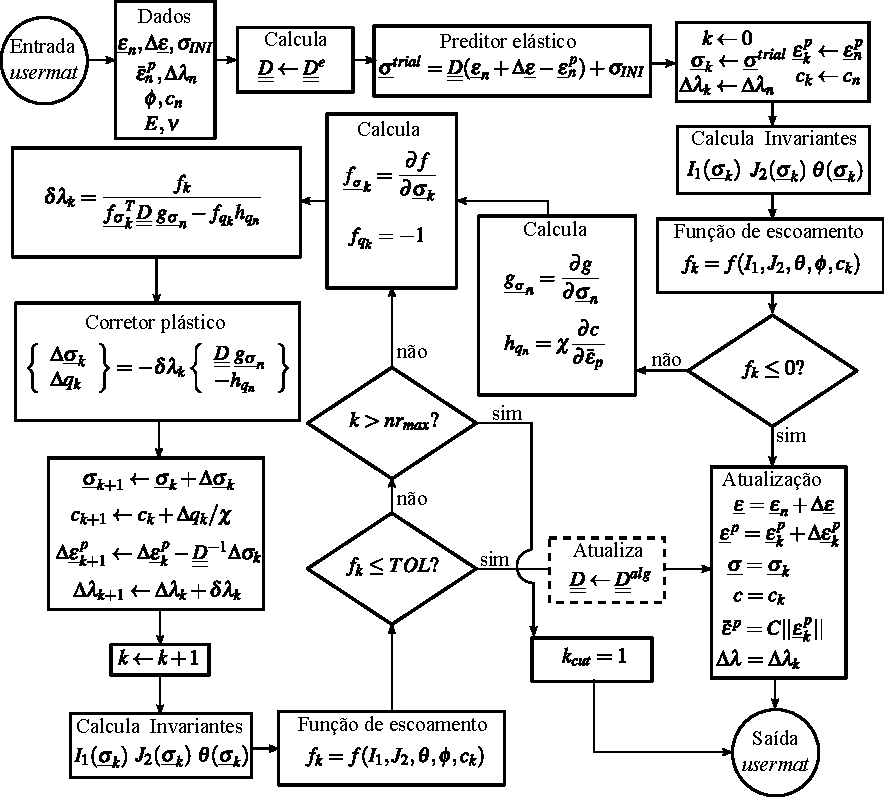
\includegraphics[scale = 1.0]{0608_4-integração EP semi-implicito.pdf}
	\end{center}
	\caption{\label{algoritmo_EP_semiimplicito}Algoritmo de integração para elastoplasticidade utilizando um esquema de Euler semi-implícito (omitindo o índice $n$+1).}
\end{figure}
No fluxograma da \autoref{algoritmo_EP_semiimplicito} aparecem três parâmetros que exigem uma explicação: $TOL$, $nr_{max}$ e $k_{cut}$. O primeiro diz respeito a tolerância exigida para o $f$ que indicará que houve a convergência do Newton-Raphson local. Como se trata de um processo iterativo o $f_k=0$ não é necessariamente atingido. Dessa forma, foi utilizado uma tolerância $TOL = 10^{-14}$. O segundo parâmetro diz respeito ao limite máximo de iterações locais que indicará a não convergência. O valor escolhido foi $nr_{max} = 10000$. Por fim, o último parâmetro $k_{cut}$ é de suma importância, pois seu valor igual a unidade indicará para o ANSYS que é necessário dividir o passo pela metade e repetir o processo de modo a buscar a convergência. Também nesse fluxograma aparece as tensões iniciais $\sigma_{INI}$ que são adicionadas ao preditor elástico.

Como visto no fluxograma da \autoref{NR-fluxograma}, após a atualização das tensões e variáveis internas tem-se a possibilidade de atualizar o módulo constitutivo. É possível utilizar o módulo tangente consistente com a linearização feita durante o algoritmo de integração das leis constitutivas (por isso também esse módulo é conhecido como módulo algorítmico). Como comentado no \autoref{cap: solução do sistema} sua utilização aumenta a taxa de convergência das iterações de equilíbrio. Sua expressão geral é definida por:
\begin{equation}
	\label{eq:D_alg1}
	\Dll^{alg} = \left(\dfrac{d\sigmal}{d\varepsilonl} \right)_{n+1}.
\end{equation}

Para derivar a expressão de $\Dll^{alg}$  escreve-se (\ref{eq:constitutiva_ep})$_{1,2,3,4}$ na sua forma incremental e resolve-se para $d\sigmal/d\varepsilonl$  \cite[p. 285]{Belytschko2000}. Com isso, tem-se, para a elastoplasticidade, a seguinte relação (omitindo-se o índice $n+1$):
\begin{equation}
	\label{eq:D_alg_ep}
	\Dll^{alg} = \Dll - \dfrac{\Dll~\dgdsl_n~\dfdsl^T \Dll}{\dfdsl^T\Dll~\dgdsl_n-\dfdql \hl_n}
\end{equation}
Adotar o módulo tangente consistente faz com que a convergência seja atingida com menos iterações de equilíbrio globais, contudo, o procedimento tem um custo para sistemas grandes, uma vez que a cada iteração é exigida a montagem e fatorização da matriz de rigidez global (caso seja utilizado a opção de Newton-Raphson Completo).  Portanto, é comum para sistemas grandes utilizar o módulo elástico $\Dll \leftarrow \Dll^e$. No presente trabalho essa atualização foi implementada, é opcional e controlada por um parâmetro.

\subsection{Integração das equações constitutivas viscoplásticas}

Como visto no \autoref{cap: modelo mecanico}, considerando a hipótese das transformações infinitesimais, as equações constitutivas da viscoplasticidade, já na notação de Voigt, podem ser escritas como:
\begin{equation}
	\label{eq:constitutiva_vp}
	\left\{
	\begin{array}{lcl}
		\dot \sigmal = \Dll~\dot \varepsilonl^e = \Dll(\dot \varepsilonl - \dot \varepsilonl^{vp}) \\
		\dot \varepsilonl^{vp} = \dot \lambda \dgdsl \\
		\dot \ql = \dot \lambda \hl \\
		\dot f = \dfdsl^T \dot \sigmal + \dfdql^T \dot \ql = 0 \\
		\dot \lambda =  \dfrac{\Phi(\sigmal, \ql)}{\eta}	
	\end{array}
	\right..
\end{equation}

Tal como na elastoplasticidade, aqui também se emprega um algoritmo de integração explícito, implícito ou semi-implícito para apartir de $\left\{ \varepsilonl_n, \varepsilonl_n^{vp},\sigmal_n,\ql_n \right\}$ e do incremento de deformação total acumulado $\Delta \varepsilonl_n$ chegar aos valores $\left\{ \varepsilonl_{n+1}, \varepsilonl_{n+1}^{vp},\sigmal_{n+1},\ql_{n+1} \right\}$  da iteração seguinte $n+1$. Contudo, na viscoplasticidade não há mais a imposição da condição de consistência, ou seja, que $f_{n+1} = 0$. O que faz com que os algoritmos sejam mais simples, porém, devem obedecer certos limites de discretização para garantir a precisão.

Diferentes algoritmos de integração para viscoplasticidade podem ser encontrados na literatura, tais como em \citeonline{Cormeau1975}, \citeonline{Zienkiewicz1974},  \citeonline{Hughes1978}, \citeonline{Marques1983}, \citeonline{Peirce1984}, \citeonline{Bernaud1991}, \citeonline{Belytschko2000}, \citeonline{Neto2008} e \citeonline{Smith2014}.

Para o presente trabalho é utilizado um esquema introduzido por \citeonline{Peirce1984} conhecido como método da taxa do módulo tangente (\textit{Rate Tangente Modulus Method}), descrito em \citeonline[p. 290]{Belytschko2000}, que compreende um esquema de Euler explícito para todas as variáveis, exceto $\Delta \lambda$ que é integrado de acordo com a regra trapezoidal generalizada. Portanto, de (\ref{eq:constitutiva_vp}) tem-se:
\begin{equation}
	\label{eq:esquema_int_constitutiva_vp}
	\left\{
	\begin{array}{lcl}
		\varepsilonl_{n+1} = \varepsilonl_n + \Delta \varepsilonl \\
		\varepsilonl_{n+1}^{vp} = \varepsilonl_n^{vp} + \Delta \lambda \dgdsl_n \\
		\ql_{n+1} = \ql_n + \Delta \lambda \hl_n \\	
		\sigmal_{n+1} = \Dll~\varepsilonl_{n+1}^e = \Dll(\varepsilonl_{n+1} - \varepsilonl_{n+1}^{vp}) \\
		\Delta \lambda = \dfrac{\Delta t}{\eta}[(1-\Theta)\Phi_n + \Theta \Phi_{n+1}]
	\end{array}
	\right..
\end{equation}
em que a função de sobretensão $\Phi_{n+1}$ é obtida através da seguinte linearização:
\begin{equation}
	\label{eq:esquema_int_constitutiva_vp1}
	\Phi_{n+1} = \Phi_n + \dPhidsl_n^T \Delta \sigmal + \dPhidql_n^T \Delta \ql
\end{equation}
sendo $\dPhidsl = \partial \Phi / \partial \sigmal$ e $\dPhidql = \partial \Phi / \partial \ql$. Substituindo (\ref{eq:esquema_int_constitutiva_vp1}) em (\ref{eq:esquema_int_constitutiva_vp})$_5$ tem-se:
\begin{equation}
	\label{eq:esquema_int_constitutiva_vp2}
	\Delta \lambda = \dfrac{\Delta t}{\eta} \Phi_n + \dfrac{\theta \Delta t}{\eta}(\dPhidsl_n^T \Delta \sigmal + \dPhidql_n^T \Delta \ql).
\end{equation}

Introduzindo (\ref{eq:esquema_int_constitutiva_vp})$_2$ em (\ref{eq:esquema_int_constitutiva_vp})$_4$ e reescrevendo (\ref{eq:esquema_int_constitutiva_vp})$_3$ tem-se, na forma compacta:
\begin{equation}
	\label{eq:esquema_int_constitutiva_vp3}
	\left\{ \begin{array}{lcl} \Delta \sigmal \\ \Delta \ql \end{array} \right\} = \left\{ \begin{array}{ccc} \Dll(\Delta\varepsilonl -\Delta \lambda \dgdsl_n) \\ \Delta \lambda \hl_n \end{array} \right\}.
\end{equation}
Substituindo (\ref{eq:esquema_int_constitutiva_vp3}) em (\ref{eq:esquema_int_constitutiva_vp2}) e isolando $\Delta \lambda$ tem-se:
\begin{equation}
	\label{eq:esquema_int_constitutiva_vp4}
	\Delta \lambda = \dfrac{\Phi_n + \Theta \dPhidsl_n^T\Dll\Delta\varepsilonl}{\dfrac{\eta}{\Delta t} + \Theta (\dPhidsl_n^T\Dll~\dgdsl_n - \dPhidql_n^T \hl_n)}.
\end{equation}

Quando $0 < \Theta < 1$  tem-se um algoritmo semi-implicito e quando $\Theta = 0$ tem-se um algoritmo totalmente explícito, com $\Delta \lambda = \Delta t \dfrac{\Phi_n}{\eta}$. Como pode-se ver nessa dedução, ao contrário da integração da relação constitutiva em elastoplasticidade, não há necessidade de resolver o sistema de forma iterativa. E, além disso, todas as variáveis são obtidas do subpasso anterior $n$. Esse fato, como será visto na próxima seção, facilitará o acoplamento entre o algoritmo de viscoplasticidade e elastoplasticidade. Além disso, para viscoplasticidade não é utilizado leis de endurecimento/amolecimento, simplificando a expressão (\ref{eq:esquema_int_constitutiva_vp4}) para:
\begin{equation}
	\label{eq:esquema_int_constitutiva_vp5}
	\Delta \lambda = \dfrac{\Phi_n + \Theta \dPhidsl_n^T\Dll\Delta\varepsilonl_n}{\dfrac{\eta}{\Delta t} + \Theta \dPhidsl_n^T\Dll\dgdsl_n}.
\end{equation}

Substituindo (\ref{eq:esquema_int_constitutiva_vp5}) em (\ref{eq:esquema_int_constitutiva_vp3})$_1$ tem-se uma expressão fechada para a atualização das tensões:
\begin{equation}
	\label{eq:esquema_int_constitutiva_vp6}
	\Delta \sigmal = \Dll^{alg} \Delta \varepsilonl - \underline p
\end{equation}
em que,
\begin{equation}
	\label{eq:esquema_int_constitutiva_vp6}
	\Dll^{alg} = \Dll - \dfrac{\Theta \Dll~\dgdsl_n~\dPhidsl_n^T \Dll}{\eta/\Delta t+ \Theta \dPhidsl_n^T\Dll~\dgdsl_n},~~~\underline p = \dfrac{\Phi_n \Dll ~\dgdsl_n}{\eta/\Delta t+ \Theta \dPhidsl_n^T\Dll~\dgdsl_n}
\end{equation}

sendo $\Dll^{alg}$ o módulo constitutivo algorítmico e $\underline p$ uma pseudo-tensão que independe do incremento de deformação total.

O esquema de integração representado por (\ref{eq:esquema_int_constitutiva_vp})$_5$ é incondicionalmente estável para valor de $\Theta \geq 1/2$. Contudo, isso não garante a precisão da solução. Dessa forma, tal como para valores $\Theta < 1/2$ deve-se utilizar um valor limite para o incremento de tempo $\Delta t \leq \Delta t_{\text{lim}}$. Esse limite de uma forma geral pode ser obtido reduzindo o incremento de tempo até que a solução não varie. A rigor depende dos parâmetros do material, do esquema de integração, da superfície de escoamento e da regra de fluxo e existem algumas soluções analíticas para as superfícies clássicas. Para evitar esse problema de precisão, nesse trabalho, utilizaram-se os limites de \citeonline[p. 829]{Cormeau1975}, em que para superfície de Drucker-Prager tem-se:
\begin{equation}
	\label{eq:deltatmin_dp}
	\Delta t_{\text{lim}} \leq \left\{ 
		\begin{array}{lcl} 
			\dfrac{4}{3}\dfrac{\eta}{\Phi}\dfrac{(1+\nu)}{E} {\sqrt{3J_2}} \\
			\dfrac{\eta f_0}{\Phi'}\dfrac{(1+\nu)(1-2\nu)}{E}\dfrac{(3-\sin{\phi})^2}{\frac{3}{4}(1-2\nu)(3-\sin{\phi})^2 + 6(1+\nu)\sin{\phi}^2}
		\end{array} \right.
\end{equation}
em que $\phi'= \dfrac{d \phi}{d(f/f0)} = n(f/f0)^{n-1}$. Quando $\phi = 0$ tem-se o caso específico para a superfície de von-Mises. Esse limite é deduzido considerando viscoplasticidade associada e com esquema de integração totalmente explícito. O fluxograma para o algoritmo de integração das equações viscoplásticas pode ser visto na \autoref{algoritmo_VP_semiimplicito}.
\begin{figure}[H]
	\begin{center}
		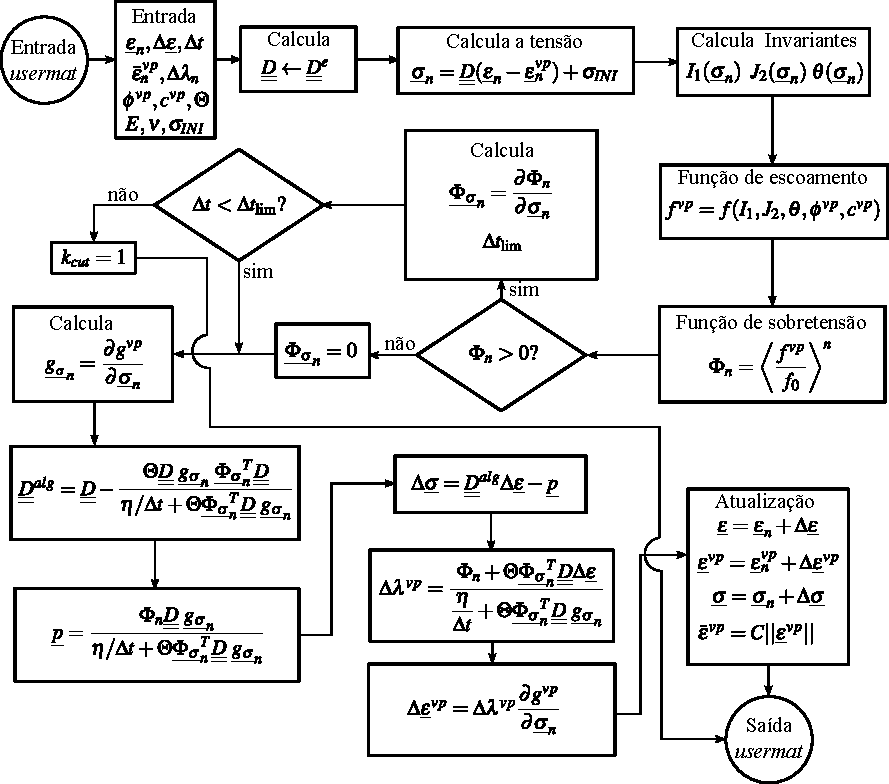
\includegraphics[scale = 1.0]{0609_4-integração VP semi-implicito sem endurecimento.pdf}
	\end{center}
	\caption{\label{algoritmo_VP_semiimplicito}Algoritmo de integração para viscoplasticidade utilizando um esquema de Euler semi-implícito ou totalmente explícito (quando $\Theta = 0$) sem endurecimento/amolecimento (omitindo o índice $n+1$).}
\end{figure}

\subsection{Integração das equações constitutivas acopladas elastoplástica-viscoplásticas}
Como visto no \autoref{cap: modelo mecanico}, considerando a hipótese das transformações infinitesimais, as equações constitutivas da elastoplasticidade e viscoplasticidade são acopladas em série de forma a obter a relação constitutiva elastoplástica-viscoplástica linearizada (\ref{eq:lei_epvp}). Além disso, como a viscoplasticidade é integrada através de uma regra semi-implícita na qual todas as incógnitas são calculadas com as variáveis conhecidas do subpasso anterior $n$, o incremento de deformação viscoplástica pode ser descontado diretamente do incremento de deformação total na etapa de predição elástica do algoritmo de elastoplasticidade.

O algoritmo para integração das equações constitutivas elastoplástica-viscoplástica pode ser visto no fluxograma da \autoref{algoritmo_EPVP}. A sua programação em \textit{Fortran} pode ser vista no Apêndice B. O procedimento para incluir essa subrotina no ANSYS pode ser vista em \citeonline{Quevedo2017}.
\begin{figure}[H]
	\begin{center}
		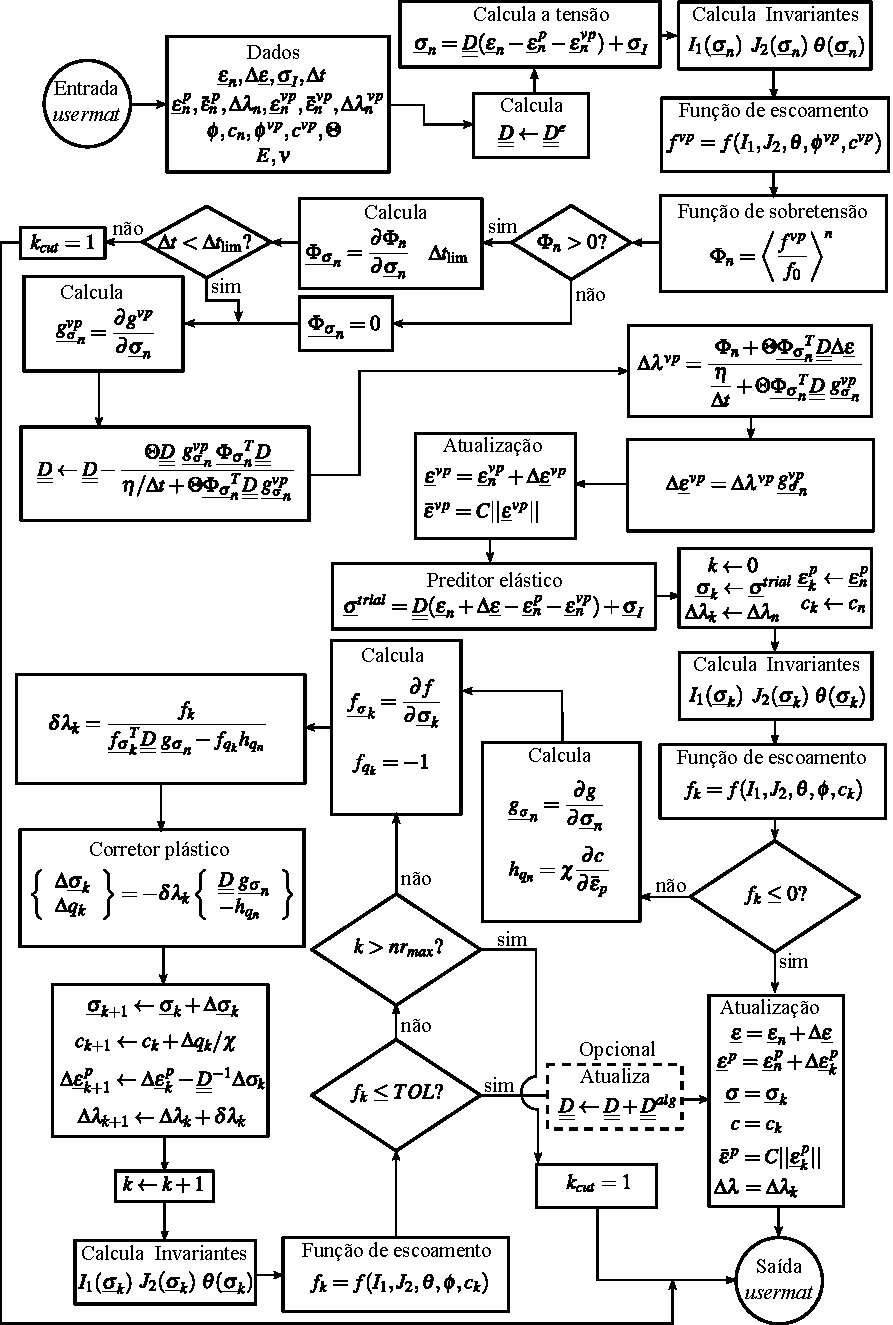
\includegraphics[scale = 1.0]{0610_5-integração EPVP.pdf}
	\end{center}
	\caption{\label{algoritmo_EPVP}Algoritmo de integração do modelo constitutivo elastoplástico-viscoplástico (omitindo o índice $n$+1).}
\end{figure}

\section{Particularizando para estado plano de deformações e axissimetria}
Em problemas tridimensionais, com materiais isotrópicos, a relação constitutiva elástica linearizada, em termos das seis componentes de tensão e de deformação pode ser escrita, na notação de Voigt, conforme (adaptado de \citeonline[p. 44]{Smith2014}):
\begin{equation}
	\label{eq:Dl}
	\left\{\begin{array}{lcl}
		\sigma_{11} \\
		\sigma_{22} \\
		\sigma_{33} \\
		\sigma_{21} \\
		\sigma_{23} \\
		\sigma_{13} 
	\end{array}\right\} = 
	\Dll
	\left\{\begin{array}{lcl}
	\varepsilon_{11} \\
	\varepsilon_{22} \\
	\varepsilon_{33} \\
	\varepsilon_{21} \\
	\varepsilon_{23} \\
	\varepsilon_{13} 
\end{array}\right\},
\end{equation}
\begin{equation}
	\Dll = 
	\dfrac{E}{(1+\nu)(1-2\nu)} 
	\begin{bmatrix}
	(1-\nu)	& \nu 		& \nu  		& 0	 		& 0 			& 0 \\
	\nu 	& (1-\nu)	& \nu  		& 0		 	& 0				& 0  \\
	\nu 	& \nu 		& (1-\nu)   & 0		 	& 0 			& 0  \\
	0		& 0			& 0		    & \dfrac{(1-2\nu)}{2} & 0 			& 0  \\
	0		& 0			& 0		    & 0	       	& \dfrac{(1-2\nu)}{2}	& 0  \\
	0		& 0			& 0		    & 0	       	& 0         	& \dfrac{(1-2\nu)}{2}
	\end{bmatrix}.
\end{equation}

Particularizando essa relação para problemas em estado plano de deformações e axissimetria tem-se (adaptado de \citeonline[p. 42]{Smith2014}):
\begin{equation}
	\label{eq:Dl}
	\left\{\begin{array}{lcl}
		\sigma_{11} \\
		\sigma_{22} \\
		\sigma_{33} \\
		\sigma_{21}
	\end{array}\right\} = \dfrac{E}{(1+\nu)(1-2\nu)}
	\begin{bmatrix}
		(1-\nu)	& \nu 		& \nu  		& 0	 		\\
		\nu 	& (1-\nu)	& \nu  		& 0		 	\\
		\nu 	& \nu 		& 1   		& 0		 	\\
		0		& 0			& 0		    & (1-2\nu)/2 
	\end{bmatrix}
	\left\{\begin{array}{lcl}
		\varepsilon_{11} \\
		\varepsilon_{22} \\
		\varepsilon_{33} \\
		\varepsilon_{21}
	\end{array}\right\}
\end{equation}
sendo que em axissimetria as direções 1, 2 e 3 correspondem respectivamente as direções $r, \theta$ e $z$ em coordenadas polares. Além disso, em problemas axissimétricos, a expressão (\ref{eq:gradiente_simetrico}) particulariza-se para (adaptado de \citeonline[p. 41]{Smith2014}):
\begin{equation}
	\label{eq:gradiente_simetrico_AXI_EPD}
	\nabla^s = 	\begin{bmatrix}
		\dfrac{\partial}{\partial r} & 0  \\
		0 & 1/r  \\
		0 & \dfrac{\partial}{\partial z} \\
		\dfrac{\partial}{\partial z} & \dfrac{\partial}{\partial r}	
	\end{bmatrix}
\end{equation}

Ademais, para o gradiente da função potencial em (\ref{eq:invariantes_tensores})$_2$, na notação de Voigt, para o caso 3D, tem-se (adaptado de \citeonline[p. 231]{Owen1980}):
\begin{equation}
	\label{eq:g1_3D}
	\gl_1 = \left\{1,1,1,0,0,0\right\}^T,
\end{equation}
\begin{equation}
	\label{eq:g2_3D}
	\gl_2 = \dfrac{1}{2\sqrt{J_2}} \left\{s_{11},s_{22},s_{33},2\sigma_{12},2\sigma_{23},2\sigma_{13}\right\}^T,
\end{equation}
\begin{equation}
	\label{eq:g3_3D}
	\gl_3 = \left\{
	\begin{array}{ccc}
	s_{22}s_{33}-\sigma_{23}^2 + J_2/3 \\
	s_{11}s_{33}-\sigma_{13}^2 + J_2/3 \\	
	s_{11}s_{22}-\sigma_{12}^2 + J_2/3 \\
	2(\sigma_{23}\sigma_{13}-s_{33}\sigma_{12}) \\
	2(\sigma_{13}\sigma_{12}-s_{11}\sigma_{23}) \\
	2(\sigma_{12}\sigma_{23}-s_{22}\sigma_{13})
	\end{array} \right\}
\end{equation}
e para o estado plano de deformações e axissimetria, tem-se (adaptado de \citeonline[p. 233]{Owen1980}):
\begin{equation}
	\label{eq:g1_2D}
	\gl_1 = \left\{1,1,1,0\right\}^T,
\end{equation}
\begin{equation}
	\label{eq:g2_2D}
	\gl_2 = \dfrac{1}{2\sqrt{J_2}} \left\{s_{11},s_{22},s_{33},2\sigma_{12}\right\}^T,
\end{equation}
\begin{equation}
	\label{eq:g3_2D}
	\gl_3 = \left\{
	\begin{array}{ccc}
		s_{22}s_{33} + J_2/3 \\
		s_{11}s_{33} + J_2/3 \\	
		s_{11}s_{22}-\sigma_{12}^2 + J_2/3 \\
		- 2s_{33}\sigma_{12}
	\end{array} \right\}.
\end{equation}

Essas expressões podem ser vistas programadas no Apêndice B entre as linhas de código 640 e 694.

\section{Domínios, discretização espacial e temporal, condições de contorno, ciclo construtivo e seus parâmetros}\label{secao_dominio}

Tal como visto na \autoref{cap:Discretização espacial em elementos finitos} o domínio $\Omega$ é discretizado em um conjunto de elementos contíguos $\Omega_e$ estabelecendo a malha de elementos finitos. No presente estudo, o domínio discretizado é o entorno de um túnel profundo, conforme \autoref{dominio_tunel}.
\begin{figure}[H]
	\begin{center}
		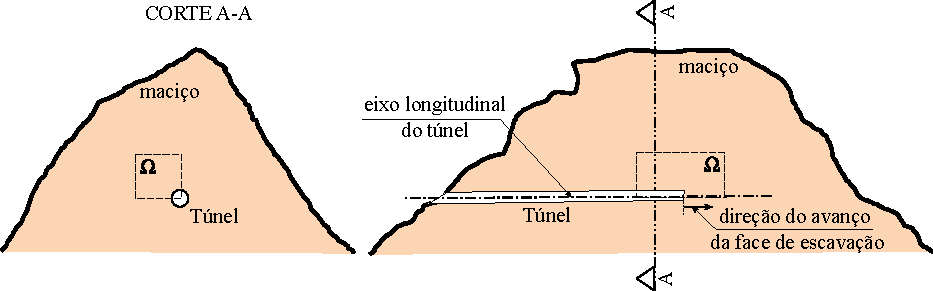
\includegraphics[scale = 1.0]{0611-dominio_do_tunel.pdf}
	\end{center}
	\caption{\label{dominio_tunel}Representação do domínio $\Omega$ a ser discretizado}
\end{figure}
As leis constitutivas vistas no \autoref{cap: modelo mecanico} são implementadas nesse domínio e estudadas em três condições: em estado plano de deformações, tridimensional e em axissimetria.

Com o intuito de obter uma malha de fácil alteração, conveniente aos estudos de convergência de malha ou análises paramétricas, o domínio foi discretizado utilizando o pré-processamento do \textit{software} ANSYS 2021R1 através da linguagem APDL (\textit{Ansys Parametric Design Language}). Com o auxílio dessa linguagem é possível controlar a discretização do domínio em função de parâmetros que podem ser alterados facilmente e, dessa forma, obtido rapidamente uma nova malha para os estudos. As discretizações apresentadas vêm da experiência obtidas em estudos anteriores \cite{Quevedo2017} considerando isoladamente a elasticidade, elastoplastcidade e viscoplasticidade do maciço. O \textit{script} APDL para a construção do modelo em axissimetria encontra-se no Apêndice A.

A \autoref{malhaEPD_tunel} apresenta o domínio para análises em estado plano de deformações com seus parâmetros, condições de contorno e malha. Como visto na \autoref{cap:Influência da escavação e o conceito de convergência da seção}, esse modelo é útil no estudo de seções fora da zona de influência da frente de escavação na qual se pode admitir a ausência de deslocamento ao longo do eixo longitudinal do túnel. Quando implementado a lei do material, esse modelo também é ideal para obter as curvas de convergência do maciço, tais como as da \autoref{cap:Método convergência-confinamento}.

Como pode-se ver na \autoref{malhaEPD_tunel}, é considerada condição de simetria para reduzir o modelo, sendo discretizada apenas uma quarta parte da região no entorno do túnel. Isso é possível em maciços homogêneos, com seção duplamente simétrica, tais como, a elíptica ou a circular ($R_{h_i}=R_{v_i}$). Também, nesse modelo, tanto a carga horizontal, vertical, bem como as tensões internas não poderão variar ao longo do domínio (condições geostáticas hidrostáticas). Como visto na \autoref{cap:Influência da profundidade do túnel}, é uma condição de estudo comum em túneis profundos. Contudo, essa condição seria facilmente modificada para considerar tensões variáveis com a profundidade e seção simétrica em torno do eixo $y$ apenas rebatendo a malha em torno do eixo $x$.

\begin{figure}[H]
	\begin{center}
		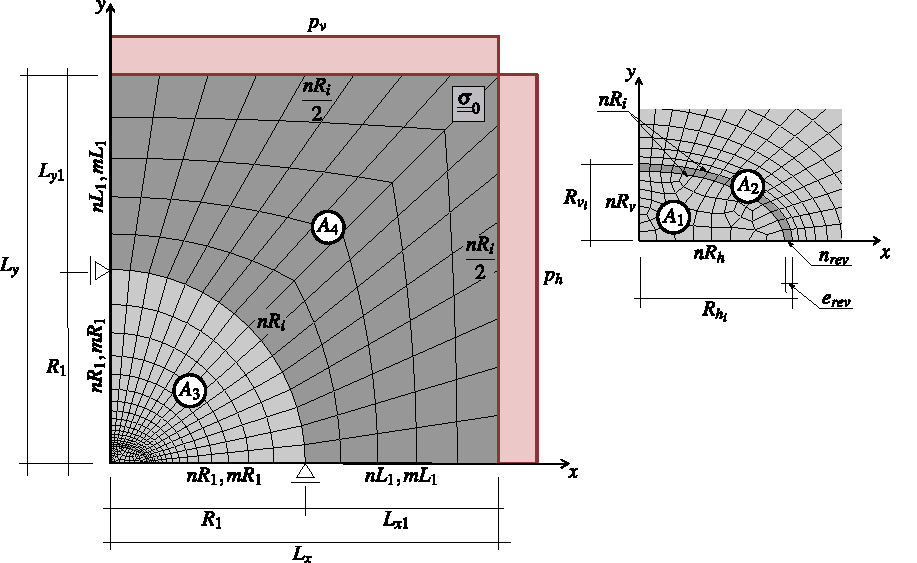
\includegraphics[scale = 1.0]{0612-malhaEPD.pdf}
	\end{center}
	\caption{\label{malhaEPD_tunel}Domínio, parâmetros geométricos, condições de contorno e malha para o modelo em estado plano de deformações}
\end{figure}

Conforme a \autoref{malhaEPD_tunel}, essa malha possui quatro regiões de refinamento: a região $A1$ representando o interior da seção do túnel, cujos elementos são desativados já no início das análises; a região $A2$ referente ao revestimento (que estará presente sempre que o parâmetro  $e_{rev} > 0$); a região $A3$, circular, no entorno do túnel onde se dará maior esforço de refinamento, pela proximidade da região escavada e, por último, a região $A4$ relativa ao restante do domínio, onde os gradientes de tensão e deformação serão pequenos. A \autoref{parametros_EPD} apresenta a definição dos parâmetros desse modelo e seus valores.

\begin{table}[H]
	\caption{Parâmetros para a construção da malha em estado plano de deformações da \autoref{malhaEPD_tunel}}
	\label{parametros_EPD}
	\centering
	\small
	\renewcommand{\arraystretch}{1.25}
	\begin{tabular}{c c c c}
		\hline
		\multicolumn{1}{c}{\textbf{PARÂMETROS}} &
		\multicolumn{1}{c}{\textbf{SÍMBOLO}} &
		\multicolumn{1}{c}{\textbf{UNIDADE}} &
		\multicolumn{1}{c}{\textbf{VALORES}} \\
		\hline
		\multicolumn{4}{c}{GEOMETRIA} \\
		\hline
		Raio horizontal na interface entre o túnel e o maciço & $R_{h_i}$ & m & 2 \\
		Raio vertical na interface entre o túnel e o maciço & $R_{v_i}$ & m & 1 \\
		Espessura do revestimento (se houver) & $e_{rev}$ & m & 0,1 \\
		Largura transversal do domínio & $L_x$ & m & 20$R_{v_i}$ \\
		Altura do domínio & $L_y$ & m & 20$R_{v_i}$ \\
		Raio da região $A3$ & $R_1$ & m & 10$R_{v_i}$ \\
		Largura além da região $A4$ & $L_{x_1}$ & m & $L_x-R_1$ \\
		Altura além da região $A4$ & $L_{y_1}$ & m & $L_y-R_1$ \\
		\hline
		\multicolumn{4}{c}{DISCRETIZAÇÃO} \\
		\hline
		Elementos na direção ortoradial & $nR_i$ & un & 10 \\
		Elementos na altura da seção escavada & $nR_{v}$ & un & $nR_i/2$ \\
		Elementos na largura da seção escavada & $nR_{h}$ & un & $nR_i/2$ \\
		Elementos na espessura do revestimento & $n_{rev}$ & un & 2 \\
		Elementos ao longo do raio da região A3 & $nR{1}$ & un & 15 \\
		Razão entre primeiro e último elemento de A3 & $mR{1}$ & adm & 15 \\
		Elementos ao longo do raio da região A4 & $nL{1}$ & un & 5 \\
		Razão entre primeiro e último elemento de A4 & $mL{1}$ & adm & 1,2 \\
		\hline
	\end{tabular}
	\normalsize
\end{table}

A discretização do domínio tridimensional faz uso dos mesmos parâmetros do estado plano de deformações, contudo, possui parâmetros adicionais para levar em consideração a dimensão ao longo do eixo longitudinal do túnel e o processo de escavação e colocação do revestimento. Esse domínio, seus parâmetros, suas condições de contorno e sua malha podem ser vistos na \autoref{malha3D_tunel} e \autoref{parametros_3D}.

\begin{figure}[H]
	\begin{center}
		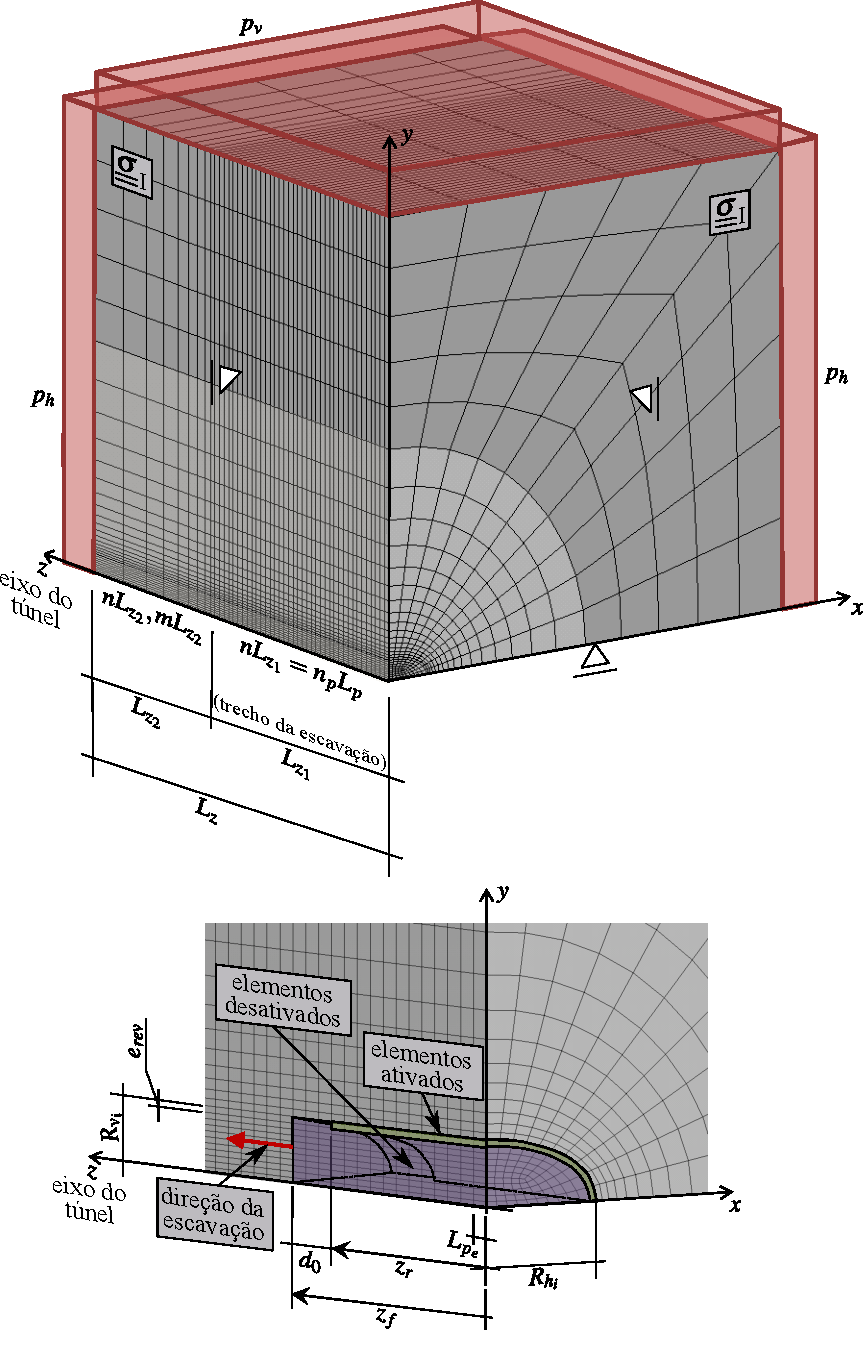
\includegraphics[scale = 1.0]{0613-malha3D.pdf}
	\end{center}
	\caption{\label{malha3D_tunel}Domínio, parâmetros geométricos, condições de contorno e malha para o modelo tridimensional}
\end{figure}

\begin{table}[H]
	\caption{Parâmetros adicionais a malha EPD para a malha em estado tridimensional de deformações da \autoref{malha3D_tunel}}
	\label{parametros_3D}
	\centering
	\small
	\renewcommand{\arraystretch}{1.25}
	\begin{tabular}{c c c c}
		\hline
		\multicolumn{1}{c}{\textbf{PARÂMETROS}} &
		\multicolumn{1}{c}{\textbf{SÍMBOLO}} &
		\multicolumn{1}{c}{\textbf{UNIDADE}} &
		\multicolumn{1}{c}{\textbf{VALORES}} \\
		\hline
		\multicolumn{4}{c}{ESCAVAÇÃO E COLOCAÇÃO DO REVESTIMENTO} \\
		\hline
		Número de passos de escavação & $n_p$ & un & 38 \\
		Número de passos na primeira escavação & $n_{p_1}$ & un & 3 \\
		Tamanho do passo de escavação & $L_{p}$ & m & $1/3R_{v_i}$ \\
		Dimensão não suportada & $d_0$ & m & $0,~2L_{p},~4L_{p}$ \\
		Cota da face do revestimento & $z_r$ & m & $(i_p-1)L_p + n_{p_1}L_p - d_0$ \\
		Cota da face de escavação & $z_f$ & m & $(i_p-1)L_p + n_{p_1}L_p$ \\
		\hline
		\multicolumn{4}{c}{GEOMETRIA} \\
		\hline
		Comprimento longitudinal do domínio & $L_z$ & m & $L_{z_1}+L_{z_2}$ \\
		Comprimento do trecho escavado & $Lz_{1}$ & m & $n_pL_p$ \\
		Comprimento do trecho não escavado & $Lz_{2}$ & m & $25L_p$ \\
		\hline
		\multicolumn{4}{c}{DISCRETIZAÇÃO} \\
		\hline
		Tamanho do elemento no trecho escavado & $L_{p_e}$ & m & $L_{p}$ \\		
		Número de elementos no trecho não escavado & $nL_{z_2}$ & un & 8 \\			
		Razão entre o primeiro e último elemento em $L_{z_2}$ & $mL_{z_2}$ & adm & 5 \\				
		\hline
	\end{tabular}
	\normalsize
\end{table}

A cada passo $1 \leq i_p \leq n_p$ de escavação é desativado os elementos até a cota da face de escavação $z_f$ e ativado os elementos do revestimento que estão defasados de $d_0$ dessa face, até a cota $z_r$. Tanto nas análises tridimensionais quanto axissimétricas, os efeitos diferidos ao longo do processo construtivo são obtidos considerando o tempo transcorrido $t_p$ durante cada passo de escavação. Esse tempo é calculado através da seguinte expressão:
\begin{equation}
	\label{eq:tp}
	t_p = \dfrac{L_p}{V_p}
\end{equation}
em que $V_p$ é a velocidade do passo em m/dias. A cada passo, conforme o \autoref{cap: solução do sistema} e a \autoref{NR-fluxograma}, esse tempo é dividido em subpassos e feita as iterações de equilíbrio de Newton-Raphson em cada subpasso. Após a convergência, segue-se o próximo passo e assim por diante. Após o término dos passos de escavação e revestimento do túnel, para os modelos dependentes do tempo, a análise roda uma série de passos até que os efeitos viscosos cessem. O incremento de tempo em cada passo é adotado como sendo metade do tempo do passo. Contudo, o método da bisseção, em busca da convergência, pode diminuir o incremento de tempo no passo.

Como pode-se notar, o modelo tridimensional possui a vantagem de considerar tanto o processo construtivo quanto seções diferentes da circular, contudo, tem um custo computacional elevado. Nesse aspecto as análises axissimétricas possuem vantagem, apesar da restrição de simetria axial. Pelo baixo custo computacional, são ideais para estudos paramétricos. O domínio para o modelo axissimétrico, seus parâmetros, condições de contorno e sua malha podem ser vistos na \autoref{malhaAXI_tunel}.

\begin{figure}[H]
	\begin{center}
		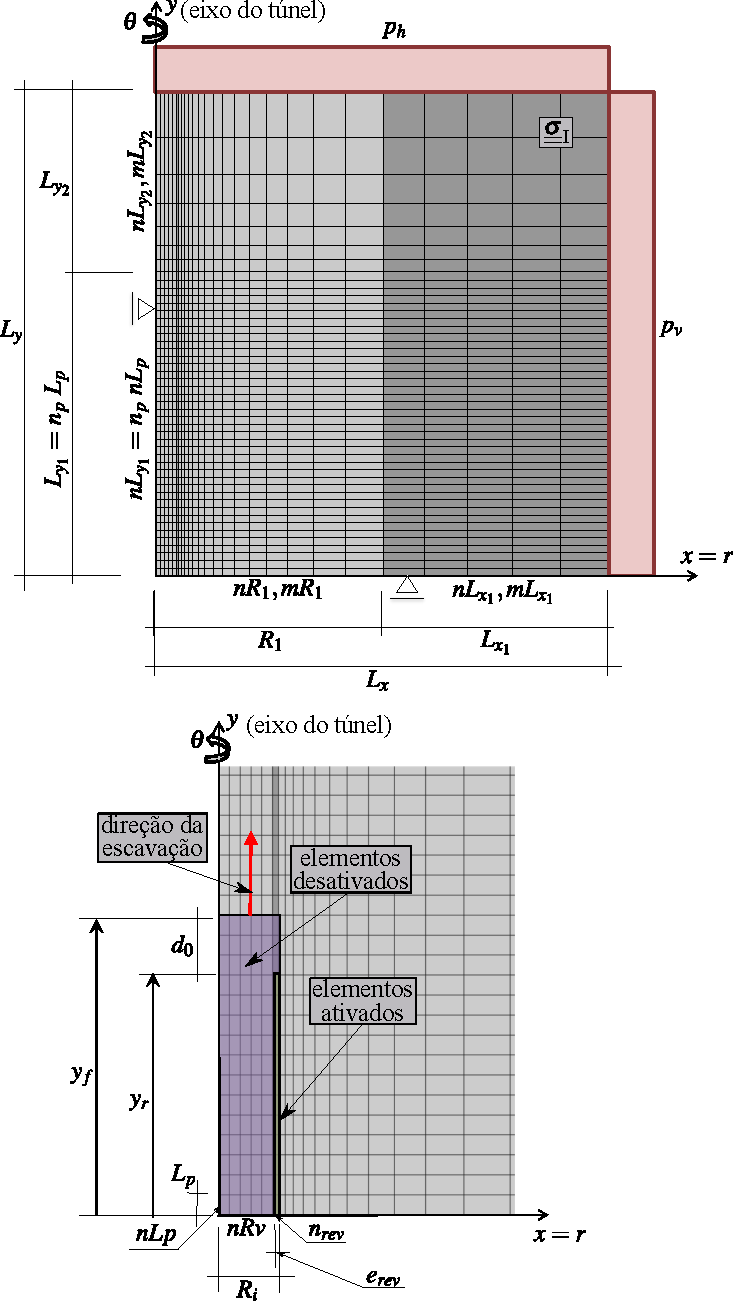
\includegraphics[scale = 1.0]{0614-malhaAXI.pdf}
	\end{center}
	\caption{\label{malhaAXI_tunel}Domínio, parâmetros geométricos, condições de contorno e malha para o modelo axissimétrico}
\end{figure}

Conforme \autoref{malhaAXI_tunel}, no modelo axissimétrico o eixo longitudinal do túnel (eixo de rotação) está ao longo do eixo $y$, enquanto que o eixo $x$ representa o eixo radial. Os parâmetros para esse modelo podem ser vistos na \autoref{parametros_AXI}.

\begin{table}[H]
	\caption{Parâmetros adicionais para a malha em estado axissimétrico \autoref{malhaAXI_tunel}}
	\label{parametros_AXI}
	\centering
	\small
	\renewcommand{\arraystretch}{1.25}
	\begin{tabular}{c c c c}
		\hline
		\multicolumn{1}{c}{\textbf{PARÂMETROS}} &
		\multicolumn{1}{c}{\textbf{SÍMBOLO}} &
		\multicolumn{1}{c}{\textbf{UNIDADE}} &
		\multicolumn{1}{c}{\textbf{VALORES}} \\
		\hline
		\multicolumn{4}{c}{GEOMETRIA} \\
		\hline
		Raio da interface entre o túnel e o maciço & $R_i$ & m & 1 \\		
		Espessura do revestimento (se houver) & $e_{rev}$ & m & 0,1 \\
		Raio total do domínio & $L_{x}$ & m & $20R_i$ \\		
		Trecho do raio além da região próxima ao túnel & $L_{x_1}$ & m & $L_x - R_1$ \\	
		Comprimento longitudinal do domínio & $L_y$ & m & $L_{y_1}+L_{y_2}$ \\
		Comprimento do trecho escavado & $Ly_{1}$ & m & $n_pL_p$ \\
		Comprimento do trecho não escavado & $Ly_{2}$ & m & $25L_p$ \\ 						
		\hline
		\multicolumn{4}{c}{ESCAVAÇÃO E COLOCAÇÃO DO REVESTIMENTO} \\
		\hline
		Número de passos de escavação & $n_p$ & un & 38 \\
		Número de passos na primeira escavação & $n_{p_i}$ & un & 3 \\
		Tamanho do passo de escavação & $L_{p}$ & m & $1/3R_{i}$ \\
		Dimensão não suportada & $d_0$ & m & $0,~2L_{p},~4L_{p}$ \\
		Cota da face do revestimento & $y_r$ & m & $(i_p-1)L_p + n_{p_i}L_p - (L_p+d_0)$ \\
		Cota da face de escavação & $y_f$ & m & $(i_p-1)L_p + n_{p_i}L_p$ \\
		\hline
		\multicolumn{4}{c}{DISCRETIZAÇÃO} \\
		\hline
		Elementos ao longo de $R_i$ & $nR_{i}$ & un & 5 \\	
		Elementos na espessura do revestimento & $n_{rev}$ & un & 2 \\			
		Elementos ao longo de $R_1$ & $nR_{1}$ & un & 15 \\	
		Razão primeiro e último elemento de $R_1$ & $mR_{1}$ & adm & 15 \\	
		Elementos ao longo de $L_{x_1}$ & $nL_{x_1}$ & un & 5 \\
		Razão primeiro e último elemento de $L_{x_1}$ & $mL_{x_1}$ & adm & 5 \\				
		Tamanho do elemento no trecho escavado & $L_{p_e}$ & m & $L_{p}$ \\	
		Número de elementos ao longo de $L_{y_2}$ & $nL_{y_2}$ & un & 8 \\			
		Razão entre o primeiro e último elemento em $L_{y_2}$ & $mL_{y_2}$ & adm & 5 \\				
		\hline
	\end{tabular}
	\normalsize
\end{table}

O \textit{script} APDL do modelo escolhido para constar no Apêndice A foi justamente o modelo axissimétrico. A entrada dos parâmetros pode ser vista entre as linhas 24 e 153 do \textit{script}.

Para simular o ciclo contrutivo de escavação e revestimento é utilizado o recurso de \textbf{ativação/desativação de elementos} em cada passo de solução. A desativação, à rigor, compreende três modificações:
\begin{alineas}
	
	\item a primeira consiste em substituir o valor do módulo de elasticidade do elemento por um valor pequeno, ou seja, 1E-12, isso fará com que durante as iterações de equilíbrio esses elementos pouco contribuam na matriz de rigidez e no incremento de forças internas, distribuindo então as tensões para os elementos vizinhos ativados;
	
	\item a segunda alteração consiste igualar a zero as tensões internas nos pontos de Gauss do elemento, que estavam acumuladas dos passos anteriores; 
	
	\item a terceira alteração consiste em igualar a zero as forças externas (se houver forças, na fronteira desses elementos) para que não entrem no cálculo do resíduo no método de Newton-Raphson.
	
\end{alineas}

No \textit{software} ANSYS esse recurso é conhecido como \textit{Birth and Death} e seu uso se dá através da seleção dos elementos e um comando APDL (EKILL e EALIVE) que identifica se estarão ativados ou desativados no passo.

O custo computacional desses modelos é refletido diretamente no tempo de processamento de cada subpasso durante a solução do sistema global. Esse tempo é função de diversos fatores. Dentre os mais simples estão a quantidade de operações em ponto flutuante (precisão simples ou dupla) necessários para a fatoração e solução do sistema frente à tecnologia de processamento (velocidade do processador e recursos de paralelização). A ordem de grandeza da quantidade de operações em ponto flutuante pode ser estimada através do tamanho do sistema. Portanto, a \autoref{tamanho_sistemas}, resume o tamanho do sistema para as malhas desses três modelos. Porém, para o tempo global, é necessário considerar as estratégias de atualização da matriz de rigidez e a quantidade de passos, sendo que este último aumenta tempo computacional linearmente.

\begin{table}[H]
	\caption{Tamanho do sistema para cada modelo}
	\label{tamanho_sistemas}
	\centering
	\small
	\renewcommand{\arraystretch}{1.25}
	\begin{tabular}{c c c c}
		\hline
		\multicolumn{1}{c}{\textbf{MODELO}} &
		\multicolumn{1}{c}{\textbf{No. ELEMENTOS}} &
		\multicolumn{1}{c}{\textbf{No. NÓS}} &
		\multicolumn{1}{c}{\textbf{SISTEMA nxn}} \\
		\hline
		EPD & 235 & 768 & 1536 \\
		3D & 13395 & 15456 & 46368 \\
		AXI & 1222 & 3813 & 7626 \\
		\hline
	\end{tabular}
	\normalsize
\end{table}

\section{Propriedades e parâmetros do modelo constitutivo}
Além dos parâmetros referente ao domínio para a construção da malha, condições de contorno e discretização do tempo tem-se os parâmetros para o modelo constitutivo do maciço e do revestimento. Como o revestimento possuí apenas comportamento elástico, ele apresenta apenas dois parâmetros $E_{rev}$ (módulo de Young) e $\nu_{rev}$ (Coeficiente de Poisson). A \autoref{parametros_EPVP} apresenta a definição dos parâmetros referente ao modelo constitutivo elastoplástico-viscoplástico.
\begin{table}[H]
	\caption{Parâmetros para o modelo constitutivo elastoplástico-viscoplástico}
	\label{parametros_EPVP}
	\centering
	\small
	\renewcommand{\arraystretch}{1.25}
	\begin{tabular}{c c c}
		\hline
		\multicolumn{1}{c}{\textbf{PARÂMETROS}} &
		\multicolumn{1}{c}{\textbf{DEFINIÇÃO}} &
		\multicolumn{1}{c}{\textbf{UNIDADE}} \\
		\hline
		\multicolumn{3}{c}{REFERENTE A PARTE ELASTICA} \\
		\hline
		E & Módulo de Young $E$  & MPa \\			
		nu & Coeficiente de Poisson $0 \leq \nu<0.5$  & adm \\		
		\hline
		\multicolumn{3}{c}{REFERENTE A PARTE ELASTOPLÁSTICA} \\
		\hline
		superficef & função de escoamento: 1-DPI, 2-DPII, 3-DPIII  & - \\		
		superficieg & função potencial: 1-DPI, 2-DPII, 3-DPIII & - \\
		fi & angulo de atrito $\phi$ (0 - VM ou TR) & graus \\		
		psi & dilatância $0<\psi<\phi$ (se $=\phi$ - plasticidade associada) & graus \\	
		ci & coesão inicial $c_i$ & MPa \\
		cp & coesão pico $c_p$ & MPa \\
		cr & coesão residual $c_r$ & MPa \\ 
		epspI & deformação equivalente que delimita a zona I $\bar \varepsilon^p_{I}$ & adm \\
		epspII & deformação equivalente que delimita a zona II $\bar \varepsilon^p_{II}$ & adm \\
		epspr & deformação equivalente que delimita a zona III $\bar \varepsilon^p_{r}$ & adm \\	
		Dalg & atualização do módulo: 0 - elástico, 1 - consistente & - \\					
		\hline
		\multicolumn{3}{c}{REFERENTE A PARTE VISCOPLASTICA} \\
		\hline
		superficefvp & função de escoamento: 1-DPI, 2-DPII, 3-DPIII  & - \\
		superficiegvp & função potencial: 1-DPI, 2-DPII, 3-DPIII & - \\
		fivp & angulo de atrito $\phi^{vp}$ (0 - VM ou TR) & graus \\
		psivp & dilatância $0<\psi^{vp}<\phi{vp}$ (se $=\phi^{vp}$ - viscoplasticidade associada) & graus \\
		cvp & coesão $c^{vp}$ & MPa \\
		n & expoente do modelo de Perzyna $n$ & adm \\
		eta & constante de viscosidade dinâmica $\eta$ & dia \\
		f0 & parâmetro de tensão a partir do qual inicia o fenômeno viscoso $f_0$ & MPa \\
		thetavp & $\Theta$: $\Theta=0$ - totalmente explícito, $0<\Theta<1$ - semi-implicito & adm \\
		\hline
	\end{tabular}
	\normalsize
\end{table}

Esse modelo constitutivo e os parâmetros entram no \textit{script} através de três comandos APDL na definição do material: TB,USER (utilizado para definir o material como sendo do usuário e onde é declarado o número total de parâmetros, no caso, 23), TBDATA (que atribui os parâmetros para o \textit{array} de propriedades do material utilizado dentro da \textit{Usermat}) e TB,STATE (que dimensiona o vetor de variáveis de estado). No Apêndice A, nas linhas 238-251, é ilustrado a declaração desse modelo constitutivo. É possível plotar algumas variáveis calculadas desse modelo através do comando APDL PLNSOL,SVAR,[componente]. As componentes são mostradas nas linhas 115-134 no Apêndice B. De maior importância talvez sejam as deformações equivalentes elastoplásticas (componente 1) e viscoplásticas (componente 6). Também, quando se tem amolecimento/endurecimento, pode ser interessante plotar a coesão (componente 3).
 
Cada comportamento (elástico, elastoplástico e viscoplástico) foi programado em separado. Contudo, o modelo constitutivo elastoplástico-viscoplástico é geral e capaz de reproduzir cada comportamento em separado dependendo do valor de alguns parâmetros. Por exemplo, ao colocar valores de coesão elevados as funções de escoamento (ora da elastoplasticidade ou viscoplasticidade) não são atingidas podendo dessa forma selecionar o comportamento apenas elástico (quando todas coesões são elevadas), elastoplástico (quando a coesão viscoplástica é elevada) ou viscoplástico (quando as coesões elastoplásticas são elevadas). Se as coesões $c_i, c_p$ e $c_r$ tiverem o mesmo valor, tem-se na parte elastoplástica um comportamento plástico perfeito.


